% Created by tikzDevice version 0.12.6 on 2025-02-16 23:19:58
% !TEX encoding = UTF-8 Unicode
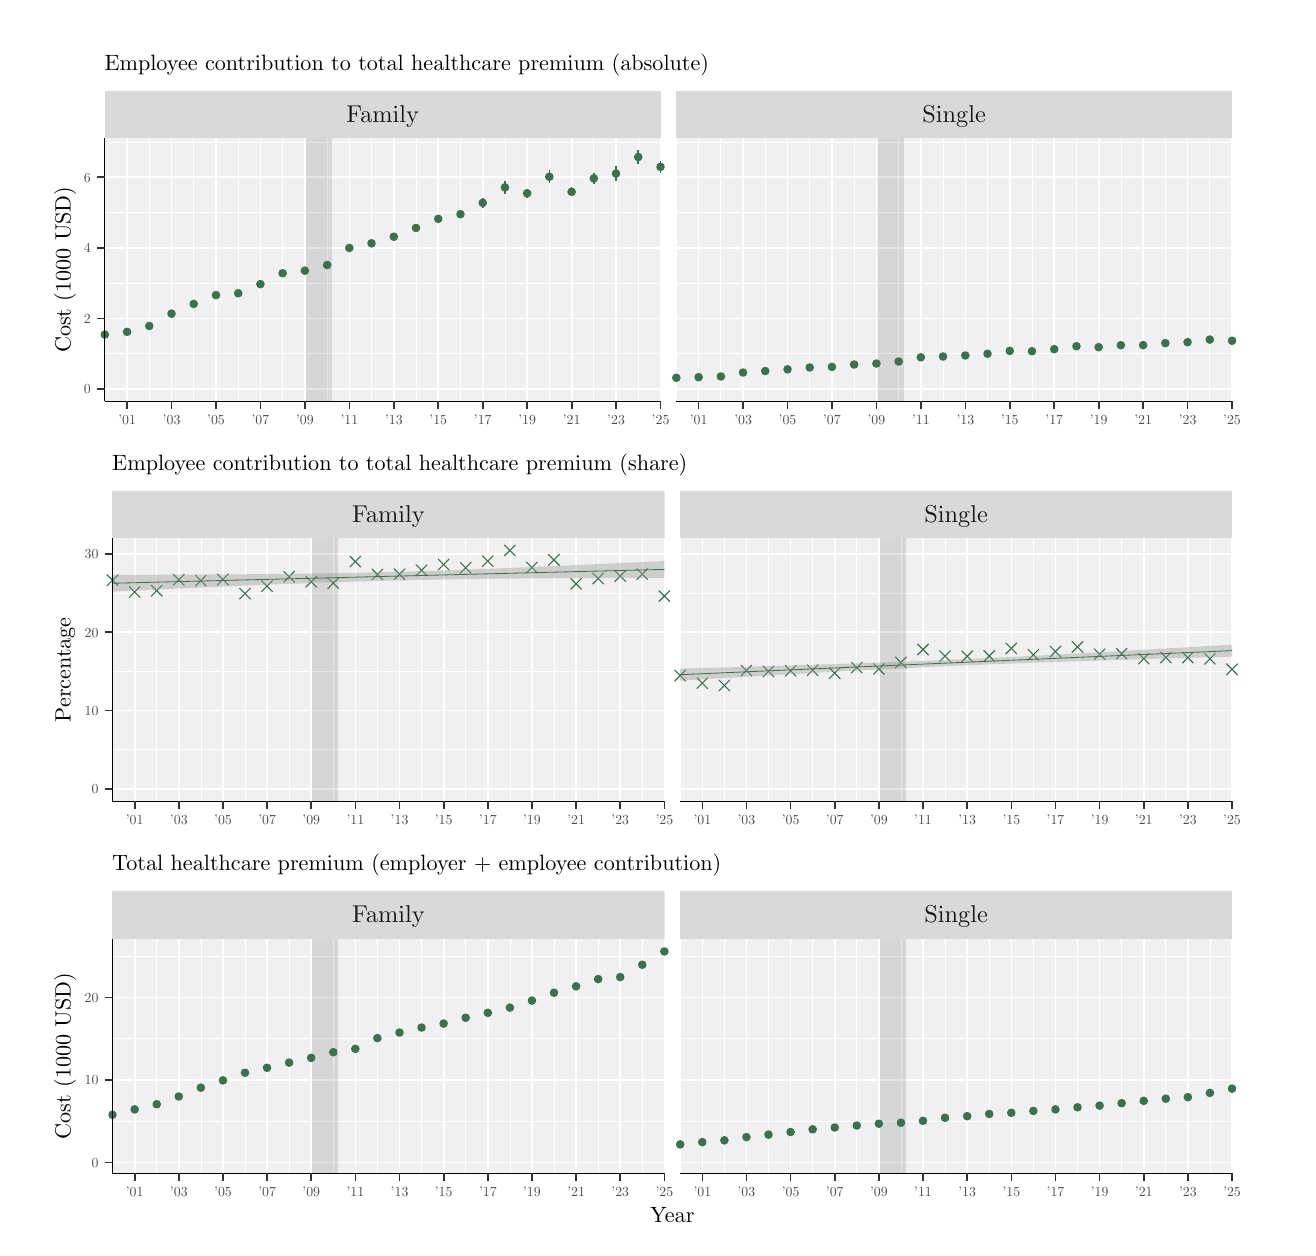
\begin{tikzpicture}[x=1pt,y=1pt]
\definecolor{fillColor}{RGB}{255,255,255}
\path[use as bounding box,fill=fillColor,fill opacity=0.00] (0,0) rectangle (455.30,433.62);
\begin{scope}
\path[clip] (  0.00,289.08) rectangle (455.30,433.62);
\definecolor{drawColor}{RGB}{255,255,255}
\definecolor{fillColor}{RGB}{255,255,255}

\path[draw=drawColor,line width= 0.6pt,line join=round,line cap=round,fill=fillColor] (  0.00,289.08) rectangle (455.30,433.62);
\end{scope}
\begin{scope}
\path[clip] (  0.00,  0.00) rectangle (455.30,433.62);
\definecolor{fillColor}{gray}{0.94}

\path[fill=fillColor] ( 27.77,298.74) rectangle (228.78,393.57);
\definecolor{drawColor}{RGB}{255,255,255}

\path[draw=drawColor,line width= 0.3pt,line join=round] ( 27.77,315.80) --
	(228.78,315.80);

\path[draw=drawColor,line width= 0.3pt,line join=round] ( 27.77,341.30) --
	(228.78,341.30);

\path[draw=drawColor,line width= 0.3pt,line join=round] ( 27.77,366.80) --
	(228.78,366.80);

\path[draw=drawColor,line width= 0.3pt,line join=round] ( 27.77,392.30) --
	(228.78,392.30);

\path[draw=drawColor,line width= 0.3pt,line join=round] ( 27.91,298.74) --
	( 27.91,393.57);

\path[draw=drawColor,line width= 0.3pt,line join=round] ( 43.97,298.74) --
	( 43.97,393.57);

\path[draw=drawColor,line width= 0.3pt,line join=round] ( 60.03,298.74) --
	( 60.03,393.57);

\path[draw=drawColor,line width= 0.3pt,line join=round] ( 76.10,298.74) --
	( 76.10,393.57);

\path[draw=drawColor,line width= 0.3pt,line join=round] ( 92.16,298.74) --
	( 92.16,393.57);

\path[draw=drawColor,line width= 0.3pt,line join=round] (108.22,298.74) --
	(108.22,393.57);

\path[draw=drawColor,line width= 0.3pt,line join=round] (124.28,298.74) --
	(124.28,393.57);

\path[draw=drawColor,line width= 0.3pt,line join=round] (140.35,298.74) --
	(140.35,393.57);

\path[draw=drawColor,line width= 0.3pt,line join=round] (156.41,298.74) --
	(156.41,393.57);

\path[draw=drawColor,line width= 0.3pt,line join=round] (172.47,298.74) --
	(172.47,393.57);

\path[draw=drawColor,line width= 0.3pt,line join=round] (188.53,298.74) --
	(188.53,393.57);

\path[draw=drawColor,line width= 0.3pt,line join=round] (204.60,298.74) --
	(204.60,393.57);

\path[draw=drawColor,line width= 0.3pt,line join=round] (220.66,298.74) --
	(220.66,393.57);

\path[draw=drawColor,line width= 0.6pt,line join=round] ( 27.77,303.05) --
	(228.78,303.05);

\path[draw=drawColor,line width= 0.6pt,line join=round] ( 27.77,328.55) --
	(228.78,328.55);

\path[draw=drawColor,line width= 0.6pt,line join=round] ( 27.77,354.05) --
	(228.78,354.05);

\path[draw=drawColor,line width= 0.6pt,line join=round] ( 27.77,379.55) --
	(228.78,379.55);

\path[draw=drawColor,line width= 0.6pt,line join=round] ( 35.95,298.74) --
	( 35.95,393.57);

\path[draw=drawColor,line width= 0.6pt,line join=round] ( 52.00,298.74) --
	( 52.00,393.57);

\path[draw=drawColor,line width= 0.6pt,line join=round] ( 68.07,298.74) --
	( 68.07,393.57);

\path[draw=drawColor,line width= 0.6pt,line join=round] ( 84.12,298.74) --
	( 84.12,393.57);

\path[draw=drawColor,line width= 0.6pt,line join=round] (100.20,298.74) --
	(100.20,393.57);

\path[draw=drawColor,line width= 0.6pt,line join=round] (116.25,298.74) --
	(116.25,393.57);

\path[draw=drawColor,line width= 0.6pt,line join=round] (132.32,298.74) --
	(132.32,393.57);

\path[draw=drawColor,line width= 0.6pt,line join=round] (148.37,298.74) --
	(148.37,393.57);

\path[draw=drawColor,line width= 0.6pt,line join=round] (164.45,298.74) --
	(164.45,393.57);

\path[draw=drawColor,line width= 0.6pt,line join=round] (180.50,298.74) --
	(180.50,393.57);

\path[draw=drawColor,line width= 0.6pt,line join=round] (196.57,298.74) --
	(196.57,393.57);

\path[draw=drawColor,line width= 0.6pt,line join=round] (212.62,298.74) --
	(212.62,393.57);

\path[draw=drawColor,line width= 0.6pt,line join=round] (228.70,298.74) --
	(228.70,393.57);
\definecolor{fillColor}{RGB}{190,190,190}

\path[fill=fillColor,fill opacity=0.01] (100.61,298.74) rectangle (110.00,393.57);

\path[fill=fillColor,fill opacity=0.01] (100.61,298.74) rectangle (110.00,393.57);

\path[fill=fillColor,fill opacity=0.01] (100.61,298.74) rectangle (110.00,393.57);

\path[fill=fillColor,fill opacity=0.01] (100.61,298.74) rectangle (110.00,393.57);

\path[fill=fillColor,fill opacity=0.01] (100.61,298.74) rectangle (110.00,393.57);

\path[fill=fillColor,fill opacity=0.01] (100.61,298.74) rectangle (110.00,393.57);

\path[fill=fillColor,fill opacity=0.01] (100.61,298.74) rectangle (110.00,393.57);

\path[fill=fillColor,fill opacity=0.01] (100.61,298.74) rectangle (110.00,393.57);

\path[fill=fillColor,fill opacity=0.01] (100.61,298.74) rectangle (110.00,393.57);

\path[fill=fillColor,fill opacity=0.01] (100.61,298.74) rectangle (110.00,393.57);

\path[fill=fillColor,fill opacity=0.01] (100.61,298.74) rectangle (110.00,393.57);

\path[fill=fillColor,fill opacity=0.01] (100.61,298.74) rectangle (110.00,393.57);

\path[fill=fillColor,fill opacity=0.01] (100.61,298.74) rectangle (110.00,393.57);

\path[fill=fillColor,fill opacity=0.01] (100.61,298.74) rectangle (110.00,393.57);

\path[fill=fillColor,fill opacity=0.01] (100.61,298.74) rectangle (110.00,393.57);

\path[fill=fillColor,fill opacity=0.01] (100.61,298.74) rectangle (110.00,393.57);

\path[fill=fillColor,fill opacity=0.01] (100.61,298.74) rectangle (110.00,393.57);

\path[fill=fillColor,fill opacity=0.01] (100.61,298.74) rectangle (110.00,393.57);

\path[fill=fillColor,fill opacity=0.01] (100.61,298.74) rectangle (110.00,393.57);

\path[fill=fillColor,fill opacity=0.01] (100.61,298.74) rectangle (110.00,393.57);

\path[fill=fillColor,fill opacity=0.01] (100.61,298.74) rectangle (110.00,393.57);

\path[fill=fillColor,fill opacity=0.01] (100.61,298.74) rectangle (110.00,393.57);

\path[fill=fillColor,fill opacity=0.01] (100.61,298.74) rectangle (110.00,393.57);

\path[fill=fillColor,fill opacity=0.01] (100.61,298.74) rectangle (110.00,393.57);

\path[fill=fillColor,fill opacity=0.01] (100.61,298.74) rectangle (110.00,393.57);

\path[fill=fillColor,fill opacity=0.01] (100.61,298.74) rectangle (110.00,393.57);
\definecolor{drawColor}{RGB}{60,113,79}

\path[draw=drawColor,line width= 0.6pt,line join=round] ( 27.88,322.09) -- ( 27.88,323.35);

\path[draw=drawColor,line width= 0.6pt,line join=round] ( 35.92,323.04) -- ( 35.92,324.34);

\path[draw=drawColor,line width= 0.6pt,line join=round] ( 43.95,325.20) -- ( 43.95,326.46);

\path[draw=drawColor,line width= 0.6pt,line join=round] ( 51.98,329.56) -- ( 51.98,331.03);

\path[draw=drawColor,line width= 0.6pt,line join=round] ( 60.00,333.07) -- ( 60.00,334.53);

\path[draw=drawColor,line width= 0.6pt,line join=round] ( 68.05,336.15) -- ( 68.05,337.80);

\path[draw=drawColor,line width= 0.6pt,line join=round] ( 76.08,336.77) -- ( 76.08,338.51);

\path[draw=drawColor,line width= 0.6pt,line join=round] ( 84.10,340.03) -- ( 84.10,341.88);

\path[draw=drawColor,line width= 0.6pt,line join=round] ( 92.13,343.83) -- ( 92.13,345.93);

\path[draw=drawColor,line width= 0.6pt,line join=round] (100.17,344.70) -- (100.17,346.92);

\path[draw=drawColor,line width= 0.6pt,line join=round] (108.20,346.84) -- (108.20,348.88);

\path[draw=drawColor,line width= 0.6pt,line join=round] (116.23,352.67) -- (116.23,355.35);

\path[draw=drawColor,line width= 0.6pt,line join=round] (124.25,354.21) -- (124.25,357.17);

\path[draw=drawColor,line width= 0.6pt,line join=round] (132.30,356.71) -- (132.30,359.44);

\path[draw=drawColor,line width= 0.6pt,line join=round] (140.32,359.91) -- (140.32,362.59);

\path[draw=drawColor,line width= 0.6pt,line join=round] (148.35,363.06) -- (148.35,366.03);

\path[draw=drawColor,line width= 0.6pt,line join=round] (156.38,364.70) -- (156.38,367.75);

\path[draw=drawColor,line width= 0.6pt,line join=round] (164.42,368.62) -- (164.42,372.04);

\path[draw=drawColor,line width= 0.6pt,line join=round] (172.45,373.61) -- (172.45,378.19);

\path[draw=drawColor,line width= 0.6pt,line join=round] (180.48,372.05) -- (180.48,375.49);

\path[draw=drawColor,line width= 0.6pt,line join=round] (188.50,377.46) -- (188.50,382.02);

\path[draw=drawColor,line width= 0.6pt,line join=round] (196.55,372.65) -- (196.55,375.94);

\path[draw=drawColor,line width= 0.6pt,line join=round] (204.57,377.20) -- (204.57,381.11);

\path[draw=drawColor,line width= 0.6pt,line join=round] (212.60,378.31) -- (212.60,383.49);

\path[draw=drawColor,line width= 0.6pt,line join=round] (220.63,384.50) -- (220.63,389.26);

\path[draw=drawColor,line width= 0.6pt,line join=round] (228.67,381.12) -- (228.67,385.52);
\definecolor{fillColor}{RGB}{60,113,79}

\path[draw=drawColor,line width= 0.8pt,line join=round,line cap=round,fill=fillColor] ( 27.88,322.72) circle (  1.14);

\path[draw=drawColor,line width= 0.8pt,line join=round,line cap=round,fill=fillColor] ( 35.92,323.69) circle (  1.14);

\path[draw=drawColor,line width= 0.8pt,line join=round,line cap=round,fill=fillColor] ( 43.95,325.83) circle (  1.14);

\path[draw=drawColor,line width= 0.8pt,line join=round,line cap=round,fill=fillColor] ( 51.98,330.29) circle (  1.14);

\path[draw=drawColor,line width= 0.8pt,line join=round,line cap=round,fill=fillColor] ( 60.00,333.80) circle (  1.14);

\path[draw=drawColor,line width= 0.8pt,line join=round,line cap=round,fill=fillColor] ( 68.05,336.98) circle (  1.14);

\path[draw=drawColor,line width= 0.8pt,line join=round,line cap=round,fill=fillColor] ( 76.08,337.64) circle (  1.14);

\path[draw=drawColor,line width= 0.8pt,line join=round,line cap=round,fill=fillColor] ( 84.10,340.95) circle (  1.14);

\path[draw=drawColor,line width= 0.8pt,line join=round,line cap=round,fill=fillColor] ( 92.13,344.88) circle (  1.14);

\path[draw=drawColor,line width= 0.8pt,line join=round,line cap=round,fill=fillColor] (100.17,345.81) circle (  1.14);

\path[draw=drawColor,line width= 0.8pt,line join=round,line cap=round,fill=fillColor] (108.20,347.86) circle (  1.14);

\path[draw=drawColor,line width= 0.8pt,line join=round,line cap=round,fill=fillColor] (116.23,354.01) circle (  1.14);

\path[draw=drawColor,line width= 0.8pt,line join=round,line cap=round,fill=fillColor] (124.25,355.69) circle (  1.14);

\path[draw=drawColor,line width= 0.8pt,line join=round,line cap=round,fill=fillColor] (132.30,358.08) circle (  1.14);

\path[draw=drawColor,line width= 0.8pt,line join=round,line cap=round,fill=fillColor] (140.32,361.25) circle (  1.14);

\path[draw=drawColor,line width= 0.8pt,line join=round,line cap=round,fill=fillColor] (148.35,364.54) circle (  1.14);

\path[draw=drawColor,line width= 0.8pt,line join=round,line cap=round,fill=fillColor] (156.38,366.22) circle (  1.14);

\path[draw=drawColor,line width= 0.8pt,line join=round,line cap=round,fill=fillColor] (164.42,370.33) circle (  1.14);

\path[draw=drawColor,line width= 0.8pt,line join=round,line cap=round,fill=fillColor] (172.45,375.90) circle (  1.14);

\path[draw=drawColor,line width= 0.8pt,line join=round,line cap=round,fill=fillColor] (180.48,373.77) circle (  1.14);

\path[draw=drawColor,line width= 0.8pt,line join=round,line cap=round,fill=fillColor] (188.50,379.74) circle (  1.14);

\path[draw=drawColor,line width= 0.8pt,line join=round,line cap=round,fill=fillColor] (196.55,374.30) circle (  1.14);

\path[draw=drawColor,line width= 0.8pt,line join=round,line cap=round,fill=fillColor] (204.57,379.15) circle (  1.14);

\path[draw=drawColor,line width= 0.8pt,line join=round,line cap=round,fill=fillColor] (212.60,380.90) circle (  1.14);

\path[draw=drawColor,line width= 0.8pt,line join=round,line cap=round,fill=fillColor] (220.63,386.88) circle (  1.14);

\path[draw=drawColor,line width= 0.8pt,line join=round,line cap=round,fill=fillColor] (228.67,383.32) circle (  1.14);
\end{scope}
\begin{scope}
\path[clip] (  0.00,  0.00) rectangle (455.30,433.62);
\definecolor{fillColor}{gray}{0.94}

\path[fill=fillColor] (234.28,298.74) rectangle (435.30,393.57);
\definecolor{drawColor}{RGB}{255,255,255}

\path[draw=drawColor,line width= 0.3pt,line join=round] (234.28,315.80) --
	(435.30,315.80);

\path[draw=drawColor,line width= 0.3pt,line join=round] (234.28,341.30) --
	(435.30,341.30);

\path[draw=drawColor,line width= 0.3pt,line join=round] (234.28,366.80) --
	(435.30,366.80);

\path[draw=drawColor,line width= 0.3pt,line join=round] (234.28,392.30) --
	(435.30,392.30);

\path[draw=drawColor,line width= 0.3pt,line join=round] (234.43,298.74) --
	(234.43,393.57);

\path[draw=drawColor,line width= 0.3pt,line join=round] (250.49,298.74) --
	(250.49,393.57);

\path[draw=drawColor,line width= 0.3pt,line join=round] (266.55,298.74) --
	(266.55,393.57);

\path[draw=drawColor,line width= 0.3pt,line join=round] (282.61,298.74) --
	(282.61,393.57);

\path[draw=drawColor,line width= 0.3pt,line join=round] (298.68,298.74) --
	(298.68,393.57);

\path[draw=drawColor,line width= 0.3pt,line join=round] (314.74,298.74) --
	(314.74,393.57);

\path[draw=drawColor,line width= 0.3pt,line join=round] (330.80,298.74) --
	(330.80,393.57);

\path[draw=drawColor,line width= 0.3pt,line join=round] (346.86,298.74) --
	(346.86,393.57);

\path[draw=drawColor,line width= 0.3pt,line join=round] (362.93,298.74) --
	(362.93,393.57);

\path[draw=drawColor,line width= 0.3pt,line join=round] (378.99,298.74) --
	(378.99,393.57);

\path[draw=drawColor,line width= 0.3pt,line join=round] (395.05,298.74) --
	(395.05,393.57);

\path[draw=drawColor,line width= 0.3pt,line join=round] (411.11,298.74) --
	(411.11,393.57);

\path[draw=drawColor,line width= 0.3pt,line join=round] (427.18,298.74) --
	(427.18,393.57);

\path[draw=drawColor,line width= 0.6pt,line join=round] (234.28,303.05) --
	(435.30,303.05);

\path[draw=drawColor,line width= 0.6pt,line join=round] (234.28,328.55) --
	(435.30,328.55);

\path[draw=drawColor,line width= 0.6pt,line join=round] (234.28,354.05) --
	(435.30,354.05);

\path[draw=drawColor,line width= 0.6pt,line join=round] (234.28,379.55) --
	(435.30,379.55);

\path[draw=drawColor,line width= 0.6pt,line join=round] (242.46,298.74) --
	(242.46,393.57);

\path[draw=drawColor,line width= 0.6pt,line join=round] (258.52,298.74) --
	(258.52,393.57);

\path[draw=drawColor,line width= 0.6pt,line join=round] (274.59,298.74) --
	(274.59,393.57);

\path[draw=drawColor,line width= 0.6pt,line join=round] (290.64,298.74) --
	(290.64,393.57);

\path[draw=drawColor,line width= 0.6pt,line join=round] (306.71,298.74) --
	(306.71,393.57);

\path[draw=drawColor,line width= 0.6pt,line join=round] (322.76,298.74) --
	(322.76,393.57);

\path[draw=drawColor,line width= 0.6pt,line join=round] (338.84,298.74) --
	(338.84,393.57);

\path[draw=drawColor,line width= 0.6pt,line join=round] (354.89,298.74) --
	(354.89,393.57);

\path[draw=drawColor,line width= 0.6pt,line join=round] (370.96,298.74) --
	(370.96,393.57);

\path[draw=drawColor,line width= 0.6pt,line join=round] (387.01,298.74) --
	(387.01,393.57);

\path[draw=drawColor,line width= 0.6pt,line join=round] (403.09,298.74) --
	(403.09,393.57);

\path[draw=drawColor,line width= 0.6pt,line join=round] (419.14,298.74) --
	(419.14,393.57);

\path[draw=drawColor,line width= 0.6pt,line join=round] (435.21,298.74) --
	(435.21,393.57);
\definecolor{fillColor}{RGB}{190,190,190}

\path[fill=fillColor,fill opacity=0.01] (307.13,298.74) rectangle (316.52,393.57);

\path[fill=fillColor,fill opacity=0.01] (307.13,298.74) rectangle (316.52,393.57);

\path[fill=fillColor,fill opacity=0.01] (307.13,298.74) rectangle (316.52,393.57);

\path[fill=fillColor,fill opacity=0.01] (307.13,298.74) rectangle (316.52,393.57);

\path[fill=fillColor,fill opacity=0.01] (307.13,298.74) rectangle (316.52,393.57);

\path[fill=fillColor,fill opacity=0.01] (307.13,298.74) rectangle (316.52,393.57);

\path[fill=fillColor,fill opacity=0.01] (307.13,298.74) rectangle (316.52,393.57);

\path[fill=fillColor,fill opacity=0.01] (307.13,298.74) rectangle (316.52,393.57);

\path[fill=fillColor,fill opacity=0.01] (307.13,298.74) rectangle (316.52,393.57);

\path[fill=fillColor,fill opacity=0.01] (307.13,298.74) rectangle (316.52,393.57);

\path[fill=fillColor,fill opacity=0.01] (307.13,298.74) rectangle (316.52,393.57);

\path[fill=fillColor,fill opacity=0.01] (307.13,298.74) rectangle (316.52,393.57);

\path[fill=fillColor,fill opacity=0.01] (307.13,298.74) rectangle (316.52,393.57);

\path[fill=fillColor,fill opacity=0.01] (307.13,298.74) rectangle (316.52,393.57);

\path[fill=fillColor,fill opacity=0.01] (307.13,298.74) rectangle (316.52,393.57);

\path[fill=fillColor,fill opacity=0.01] (307.13,298.74) rectangle (316.52,393.57);

\path[fill=fillColor,fill opacity=0.01] (307.13,298.74) rectangle (316.52,393.57);

\path[fill=fillColor,fill opacity=0.01] (307.13,298.74) rectangle (316.52,393.57);

\path[fill=fillColor,fill opacity=0.01] (307.13,298.74) rectangle (316.52,393.57);

\path[fill=fillColor,fill opacity=0.01] (307.13,298.74) rectangle (316.52,393.57);

\path[fill=fillColor,fill opacity=0.01] (307.13,298.74) rectangle (316.52,393.57);

\path[fill=fillColor,fill opacity=0.01] (307.13,298.74) rectangle (316.52,393.57);

\path[fill=fillColor,fill opacity=0.01] (307.13,298.74) rectangle (316.52,393.57);

\path[fill=fillColor,fill opacity=0.01] (307.13,298.74) rectangle (316.52,393.57);

\path[fill=fillColor,fill opacity=0.01] (307.13,298.74) rectangle (316.52,393.57);

\path[fill=fillColor,fill opacity=0.01] (307.13,298.74) rectangle (316.52,393.57);
\definecolor{drawColor}{RGB}{60,113,79}

\path[draw=drawColor,line width= 0.6pt,line join=round] (234.39,306.87) -- (234.39,307.33);

\path[draw=drawColor,line width= 0.6pt,line join=round] (242.44,307.11) -- (242.44,307.50);

\path[draw=drawColor,line width= 0.6pt,line join=round] (250.47,307.40) -- (250.47,307.75);

\path[draw=drawColor,line width= 0.6pt,line join=round] (258.49,308.74) -- (258.49,309.24);

\path[draw=drawColor,line width= 0.6pt,line join=round] (266.52,309.30) -- (266.52,309.75);

\path[draw=drawColor,line width= 0.6pt,line join=round] (274.57,309.93) -- (274.57,310.40);

\path[draw=drawColor,line width= 0.6pt,line join=round] (282.59,310.58) -- (282.59,311.07);

\path[draw=drawColor,line width= 0.6pt,line join=round] (290.62,310.80) -- (290.62,311.29);

\path[draw=drawColor,line width= 0.6pt,line join=round] (298.64,311.61) -- (298.64,312.18);

\path[draw=drawColor,line width= 0.6pt,line join=round] (306.69,311.93) -- (306.69,312.55);

\path[draw=drawColor,line width= 0.6pt,line join=round] (314.72,312.71) -- (314.72,313.25);

\path[draw=drawColor,line width= 0.6pt,line join=round] (322.74,314.12) -- (322.74,314.90);

\path[draw=drawColor,line width= 0.6pt,line join=round] (330.77,314.44) -- (330.77,315.14);

\path[draw=drawColor,line width= 0.6pt,line join=round] (338.82,314.87) -- (338.82,315.48);

\path[draw=drawColor,line width= 0.6pt,line join=round] (346.84,315.45) -- (346.84,316.12);

\path[draw=drawColor,line width= 0.6pt,line join=round] (354.87,316.45) -- (354.87,317.21);

\path[draw=drawColor,line width= 0.6pt,line join=round] (362.89,316.31) -- (362.89,317.09);

\path[draw=drawColor,line width= 0.6pt,line join=round] (370.94,317.00) -- (370.94,317.88);

\path[draw=drawColor,line width= 0.6pt,line join=round] (378.97,317.64) -- (378.97,319.39);

\path[draw=drawColor,line width= 0.6pt,line join=round] (386.99,317.75) -- (386.99,318.59);

\path[draw=drawColor,line width= 0.6pt,line join=round] (395.02,318.33) -- (395.02,319.44);

\path[draw=drawColor,line width= 0.6pt,line join=round] (403.07,318.49) -- (403.07,319.31);

\path[draw=drawColor,line width= 0.6pt,line join=round] (411.09,319.11) -- (411.09,320.11);

\path[draw=drawColor,line width= 0.6pt,line join=round] (419.12,319.46) -- (419.12,320.47);

\path[draw=drawColor,line width= 0.6pt,line join=round] (427.14,320.30) -- (427.14,321.53);

\path[draw=drawColor,line width= 0.6pt,line join=round] (435.19,319.93) -- (435.19,321.05);
\definecolor{fillColor}{RGB}{60,113,79}

\path[draw=drawColor,line width= 0.8pt,line join=round,line cap=round,fill=fillColor] (234.39,307.10) circle (  1.14);

\path[draw=drawColor,line width= 0.8pt,line join=round,line cap=round,fill=fillColor] (242.44,307.31) circle (  1.14);

\path[draw=drawColor,line width= 0.8pt,line join=round,line cap=round,fill=fillColor] (250.47,307.57) circle (  1.14);

\path[draw=drawColor,line width= 0.8pt,line join=round,line cap=round,fill=fillColor] (258.49,308.99) circle (  1.14);

\path[draw=drawColor,line width= 0.8pt,line join=round,line cap=round,fill=fillColor] (266.52,309.53) circle (  1.14);

\path[draw=drawColor,line width= 0.8pt,line join=round,line cap=round,fill=fillColor] (274.57,310.16) circle (  1.14);

\path[draw=drawColor,line width= 0.8pt,line join=round,line cap=round,fill=fillColor] (282.59,310.83) circle (  1.14);

\path[draw=drawColor,line width= 0.8pt,line join=round,line cap=round,fill=fillColor] (290.62,311.04) circle (  1.14);

\path[draw=drawColor,line width= 0.8pt,line join=round,line cap=round,fill=fillColor] (298.64,311.90) circle (  1.14);

\path[draw=drawColor,line width= 0.8pt,line join=round,line cap=round,fill=fillColor] (306.69,312.24) circle (  1.14);

\path[draw=drawColor,line width= 0.8pt,line join=round,line cap=round,fill=fillColor] (314.72,312.98) circle (  1.14);

\path[draw=drawColor,line width= 0.8pt,line join=round,line cap=round,fill=fillColor] (322.74,314.51) circle (  1.14);

\path[draw=drawColor,line width= 0.8pt,line join=round,line cap=round,fill=fillColor] (330.77,314.79) circle (  1.14);

\path[draw=drawColor,line width= 0.8pt,line join=round,line cap=round,fill=fillColor] (338.82,315.17) circle (  1.14);

\path[draw=drawColor,line width= 0.8pt,line join=round,line cap=round,fill=fillColor] (346.84,315.79) circle (  1.14);

\path[draw=drawColor,line width= 0.8pt,line join=round,line cap=round,fill=fillColor] (354.87,316.83) circle (  1.14);

\path[draw=drawColor,line width= 0.8pt,line join=round,line cap=round,fill=fillColor] (362.89,316.70) circle (  1.14);

\path[draw=drawColor,line width= 0.8pt,line join=round,line cap=round,fill=fillColor] (370.94,317.44) circle (  1.14);

\path[draw=drawColor,line width= 0.8pt,line join=round,line cap=round,fill=fillColor] (378.97,318.51) circle (  1.14);

\path[draw=drawColor,line width= 0.8pt,line join=round,line cap=round,fill=fillColor] (386.99,318.17) circle (  1.14);

\path[draw=drawColor,line width= 0.8pt,line join=round,line cap=round,fill=fillColor] (395.02,318.88) circle (  1.14);

\path[draw=drawColor,line width= 0.8pt,line join=round,line cap=round,fill=fillColor] (403.07,318.90) circle (  1.14);

\path[draw=drawColor,line width= 0.8pt,line join=round,line cap=round,fill=fillColor] (411.09,319.61) circle (  1.14);

\path[draw=drawColor,line width= 0.8pt,line join=round,line cap=round,fill=fillColor] (419.12,319.97) circle (  1.14);

\path[draw=drawColor,line width= 0.8pt,line join=round,line cap=round,fill=fillColor] (427.14,320.91) circle (  1.14);

\path[draw=drawColor,line width= 0.8pt,line join=round,line cap=round,fill=fillColor] (435.19,320.49) circle (  1.14);
\end{scope}
\begin{scope}
\path[clip] ( 27.77,393.57) rectangle (228.78,410.84);
\definecolor{fillColor}{gray}{0.85}

\path[fill=fillColor] ( 27.77,393.57) rectangle (228.78,410.84);
\definecolor{drawColor}{gray}{0.10}

\node[text=drawColor,anchor=base,inner sep=0pt, outer sep=0pt, scale=  0.88] at (128.28,399.18) {Family};
\end{scope}
\begin{scope}
\path[clip] (234.28,393.57) rectangle (435.30,410.84);
\definecolor{fillColor}{gray}{0.85}

\path[fill=fillColor] (234.28,393.57) rectangle (435.30,410.84);
\definecolor{drawColor}{gray}{0.10}

\node[text=drawColor,anchor=base,inner sep=0pt, outer sep=0pt, scale=  0.88] at (334.79,399.18) {Single};
\end{scope}
\begin{scope}
\path[clip] (  0.00,  0.00) rectangle (455.30,433.62);
\definecolor{drawColor}{RGB}{0,0,0}

\path[draw=drawColor,line width= 0.2pt,line join=round] ( 27.77,298.74) --
	(228.78,298.74);
\end{scope}
\begin{scope}
\path[clip] (  0.00,  0.00) rectangle (455.30,433.62);
\definecolor{drawColor}{gray}{0.20}

\path[draw=drawColor,line width= 0.6pt,line join=round] ( 35.95,295.99) --
	( 35.95,298.74);

\path[draw=drawColor,line width= 0.6pt,line join=round] ( 52.00,295.99) --
	( 52.00,298.74);

\path[draw=drawColor,line width= 0.6pt,line join=round] ( 68.07,295.99) --
	( 68.07,298.74);

\path[draw=drawColor,line width= 0.6pt,line join=round] ( 84.12,295.99) --
	( 84.12,298.74);

\path[draw=drawColor,line width= 0.6pt,line join=round] (100.20,295.99) --
	(100.20,298.74);

\path[draw=drawColor,line width= 0.6pt,line join=round] (116.25,295.99) --
	(116.25,298.74);

\path[draw=drawColor,line width= 0.6pt,line join=round] (132.32,295.99) --
	(132.32,298.74);

\path[draw=drawColor,line width= 0.6pt,line join=round] (148.37,295.99) --
	(148.37,298.74);

\path[draw=drawColor,line width= 0.6pt,line join=round] (164.45,295.99) --
	(164.45,298.74);

\path[draw=drawColor,line width= 0.6pt,line join=round] (180.50,295.99) --
	(180.50,298.74);

\path[draw=drawColor,line width= 0.6pt,line join=round] (196.57,295.99) --
	(196.57,298.74);

\path[draw=drawColor,line width= 0.6pt,line join=round] (212.62,295.99) --
	(212.62,298.74);

\path[draw=drawColor,line width= 0.6pt,line join=round] (228.70,295.99) --
	(228.70,298.74);
\end{scope}
\begin{scope}
\path[clip] (  0.00,  0.00) rectangle (455.30,433.62);
\definecolor{drawColor}{gray}{0.30}

\node[text=drawColor,anchor=base,inner sep=0pt, outer sep=0pt, scale=  0.50] at ( 35.95,290.34) {'01};

\node[text=drawColor,anchor=base,inner sep=0pt, outer sep=0pt, scale=  0.50] at ( 52.00,290.34) {'03};

\node[text=drawColor,anchor=base,inner sep=0pt, outer sep=0pt, scale=  0.50] at ( 68.07,290.34) {'05};

\node[text=drawColor,anchor=base,inner sep=0pt, outer sep=0pt, scale=  0.50] at ( 84.12,290.34) {'07};

\node[text=drawColor,anchor=base,inner sep=0pt, outer sep=0pt, scale=  0.50] at (100.20,290.34) {'09};

\node[text=drawColor,anchor=base,inner sep=0pt, outer sep=0pt, scale=  0.50] at (116.25,290.34) {'11};

\node[text=drawColor,anchor=base,inner sep=0pt, outer sep=0pt, scale=  0.50] at (132.32,290.34) {'13};

\node[text=drawColor,anchor=base,inner sep=0pt, outer sep=0pt, scale=  0.50] at (148.37,290.34) {'15};

\node[text=drawColor,anchor=base,inner sep=0pt, outer sep=0pt, scale=  0.50] at (164.45,290.34) {'17};

\node[text=drawColor,anchor=base,inner sep=0pt, outer sep=0pt, scale=  0.50] at (180.50,290.34) {'19};

\node[text=drawColor,anchor=base,inner sep=0pt, outer sep=0pt, scale=  0.50] at (196.57,290.34) {'21};

\node[text=drawColor,anchor=base,inner sep=0pt, outer sep=0pt, scale=  0.50] at (212.62,290.34) {'23};

\node[text=drawColor,anchor=base,inner sep=0pt, outer sep=0pt, scale=  0.50] at (228.70,290.34) {'25};
\end{scope}
\begin{scope}
\path[clip] (  0.00,  0.00) rectangle (455.30,433.62);
\definecolor{drawColor}{RGB}{0,0,0}

\path[draw=drawColor,line width= 0.2pt,line join=round] (234.28,298.74) --
	(435.30,298.74);
\end{scope}
\begin{scope}
\path[clip] (  0.00,  0.00) rectangle (455.30,433.62);
\definecolor{drawColor}{gray}{0.20}

\path[draw=drawColor,line width= 0.6pt,line join=round] (242.46,295.99) --
	(242.46,298.74);

\path[draw=drawColor,line width= 0.6pt,line join=round] (258.52,295.99) --
	(258.52,298.74);

\path[draw=drawColor,line width= 0.6pt,line join=round] (274.59,295.99) --
	(274.59,298.74);

\path[draw=drawColor,line width= 0.6pt,line join=round] (290.64,295.99) --
	(290.64,298.74);

\path[draw=drawColor,line width= 0.6pt,line join=round] (306.71,295.99) --
	(306.71,298.74);

\path[draw=drawColor,line width= 0.6pt,line join=round] (322.76,295.99) --
	(322.76,298.74);

\path[draw=drawColor,line width= 0.6pt,line join=round] (338.84,295.99) --
	(338.84,298.74);

\path[draw=drawColor,line width= 0.6pt,line join=round] (354.89,295.99) --
	(354.89,298.74);

\path[draw=drawColor,line width= 0.6pt,line join=round] (370.96,295.99) --
	(370.96,298.74);

\path[draw=drawColor,line width= 0.6pt,line join=round] (387.01,295.99) --
	(387.01,298.74);

\path[draw=drawColor,line width= 0.6pt,line join=round] (403.09,295.99) --
	(403.09,298.74);

\path[draw=drawColor,line width= 0.6pt,line join=round] (419.14,295.99) --
	(419.14,298.74);

\path[draw=drawColor,line width= 0.6pt,line join=round] (435.21,295.99) --
	(435.21,298.74);
\end{scope}
\begin{scope}
\path[clip] (  0.00,  0.00) rectangle (455.30,433.62);
\definecolor{drawColor}{gray}{0.30}

\node[text=drawColor,anchor=base,inner sep=0pt, outer sep=0pt, scale=  0.50] at (242.46,290.34) {'01};

\node[text=drawColor,anchor=base,inner sep=0pt, outer sep=0pt, scale=  0.50] at (258.52,290.34) {'03};

\node[text=drawColor,anchor=base,inner sep=0pt, outer sep=0pt, scale=  0.50] at (274.59,290.34) {'05};

\node[text=drawColor,anchor=base,inner sep=0pt, outer sep=0pt, scale=  0.50] at (290.64,290.34) {'07};

\node[text=drawColor,anchor=base,inner sep=0pt, outer sep=0pt, scale=  0.50] at (306.71,290.34) {'09};

\node[text=drawColor,anchor=base,inner sep=0pt, outer sep=0pt, scale=  0.50] at (322.76,290.34) {'11};

\node[text=drawColor,anchor=base,inner sep=0pt, outer sep=0pt, scale=  0.50] at (338.84,290.34) {'13};

\node[text=drawColor,anchor=base,inner sep=0pt, outer sep=0pt, scale=  0.50] at (354.89,290.34) {'15};

\node[text=drawColor,anchor=base,inner sep=0pt, outer sep=0pt, scale=  0.50] at (370.96,290.34) {'17};

\node[text=drawColor,anchor=base,inner sep=0pt, outer sep=0pt, scale=  0.50] at (387.01,290.34) {'19};

\node[text=drawColor,anchor=base,inner sep=0pt, outer sep=0pt, scale=  0.50] at (403.09,290.34) {'21};

\node[text=drawColor,anchor=base,inner sep=0pt, outer sep=0pt, scale=  0.50] at (419.14,290.34) {'23};

\node[text=drawColor,anchor=base,inner sep=0pt, outer sep=0pt, scale=  0.50] at (435.21,290.34) {'25};
\end{scope}
\begin{scope}
\path[clip] (  0.00,  0.00) rectangle (455.30,433.62);
\definecolor{drawColor}{RGB}{0,0,0}

\path[draw=drawColor,line width= 0.2pt,line join=round] ( 27.77,298.74) --
	( 27.77,393.57);
\end{scope}
\begin{scope}
\path[clip] (  0.00,  0.00) rectangle (455.30,433.62);
\definecolor{drawColor}{gray}{0.30}

\node[text=drawColor,anchor=base east,inner sep=0pt, outer sep=0pt, scale=  0.50] at ( 22.82,301.33) {0};

\node[text=drawColor,anchor=base east,inner sep=0pt, outer sep=0pt, scale=  0.50] at ( 22.82,326.83) {2};

\node[text=drawColor,anchor=base east,inner sep=0pt, outer sep=0pt, scale=  0.50] at ( 22.82,352.33) {4};

\node[text=drawColor,anchor=base east,inner sep=0pt, outer sep=0pt, scale=  0.50] at ( 22.82,377.83) {6};
\end{scope}
\begin{scope}
\path[clip] (  0.00,  0.00) rectangle (455.30,433.62);
\definecolor{drawColor}{gray}{0.20}

\path[draw=drawColor,line width= 0.6pt,line join=round] ( 25.02,303.05) --
	( 27.77,303.05);

\path[draw=drawColor,line width= 0.6pt,line join=round] ( 25.02,328.55) --
	( 27.77,328.55);

\path[draw=drawColor,line width= 0.6pt,line join=round] ( 25.02,354.05) --
	( 27.77,354.05);

\path[draw=drawColor,line width= 0.6pt,line join=round] ( 25.02,379.55) --
	( 27.77,379.55);
\end{scope}
\begin{scope}
\path[clip] (  0.00,  0.00) rectangle (455.30,433.62);
\definecolor{drawColor}{RGB}{0,0,0}

\node[text=drawColor,rotate= 90.00,anchor=base,inner sep=0pt, outer sep=0pt, scale=  0.80] at ( 15.51,346.15) {Cost (1000 USD)};
\end{scope}
\begin{scope}
\path[clip] (  0.00,  0.00) rectangle (455.30,433.62);
\definecolor{drawColor}{RGB}{0,0,0}

\node[text=drawColor,anchor=base west,inner sep=0pt, outer sep=0pt, scale=  0.80] at ( 27.77,418.11) {Employee contribution to total healthcare premium (absolute)};
\end{scope}
\begin{scope}
\path[clip] (  0.00,144.54) rectangle (455.30,289.08);
\definecolor{drawColor}{RGB}{255,255,255}
\definecolor{fillColor}{RGB}{255,255,255}

\path[draw=drawColor,line width= 0.6pt,line join=round,line cap=round,fill=fillColor] (  0.00,144.54) rectangle (455.30,289.08);
\end{scope}
\begin{scope}
\path[clip] (  0.00,  0.00) rectangle (455.30,433.62);
\definecolor{fillColor}{gray}{0.94}

\path[fill=fillColor] ( 30.56,154.20) rectangle (230.18,249.03);
\definecolor{drawColor}{RGB}{255,255,255}

\path[draw=drawColor,line width= 0.3pt,line join=round] ( 30.56,172.66) --
	(230.18,172.66);

\path[draw=drawColor,line width= 0.3pt,line join=round] ( 30.56,200.97) --
	(230.18,200.97);

\path[draw=drawColor,line width= 0.3pt,line join=round] ( 30.56,229.28) --
	(230.18,229.28);

\path[draw=drawColor,line width= 0.3pt,line join=round] ( 30.70,154.20) --
	( 30.70,249.03);

\path[draw=drawColor,line width= 0.3pt,line join=round] ( 46.65,154.20) --
	( 46.65,249.03);

\path[draw=drawColor,line width= 0.3pt,line join=round] ( 62.60,154.20) --
	( 62.60,249.03);

\path[draw=drawColor,line width= 0.3pt,line join=round] ( 78.55,154.20) --
	( 78.55,249.03);

\path[draw=drawColor,line width= 0.3pt,line join=round] ( 94.50,154.20) --
	( 94.50,249.03);

\path[draw=drawColor,line width= 0.3pt,line join=round] (110.45,154.20) --
	(110.45,249.03);

\path[draw=drawColor,line width= 0.3pt,line join=round] (126.40,154.20) --
	(126.40,249.03);

\path[draw=drawColor,line width= 0.3pt,line join=round] (142.36,154.20) --
	(142.36,249.03);

\path[draw=drawColor,line width= 0.3pt,line join=round] (158.31,154.20) --
	(158.31,249.03);

\path[draw=drawColor,line width= 0.3pt,line join=round] (174.26,154.20) --
	(174.26,249.03);

\path[draw=drawColor,line width= 0.3pt,line join=round] (190.21,154.20) --
	(190.21,249.03);

\path[draw=drawColor,line width= 0.3pt,line join=round] (206.16,154.20) --
	(206.16,249.03);

\path[draw=drawColor,line width= 0.3pt,line join=round] (222.11,154.20) --
	(222.11,249.03);

\path[draw=drawColor,line width= 0.6pt,line join=round] ( 30.56,158.51) --
	(230.18,158.51);

\path[draw=drawColor,line width= 0.6pt,line join=round] ( 30.56,186.82) --
	(230.18,186.82);

\path[draw=drawColor,line width= 0.6pt,line join=round] ( 30.56,215.13) --
	(230.18,215.13);

\path[draw=drawColor,line width= 0.6pt,line join=round] ( 30.56,243.44) --
	(230.18,243.44);

\path[draw=drawColor,line width= 0.6pt,line join=round] ( 38.68,154.20) --
	( 38.68,249.03);

\path[draw=drawColor,line width= 0.6pt,line join=round] ( 54.62,154.20) --
	( 54.62,249.03);

\path[draw=drawColor,line width= 0.6pt,line join=round] ( 70.58,154.20) --
	( 70.58,249.03);

\path[draw=drawColor,line width= 0.6pt,line join=round] ( 86.52,154.20) --
	( 86.52,249.03);

\path[draw=drawColor,line width= 0.6pt,line join=round] (102.48,154.20) --
	(102.48,249.03);

\path[draw=drawColor,line width= 0.6pt,line join=round] (118.42,154.20) --
	(118.42,249.03);

\path[draw=drawColor,line width= 0.6pt,line join=round] (134.39,154.20) --
	(134.39,249.03);

\path[draw=drawColor,line width= 0.6pt,line join=round] (150.33,154.20) --
	(150.33,249.03);

\path[draw=drawColor,line width= 0.6pt,line join=round] (166.29,154.20) --
	(166.29,249.03);

\path[draw=drawColor,line width= 0.6pt,line join=round] (182.23,154.20) --
	(182.23,249.03);

\path[draw=drawColor,line width= 0.6pt,line join=round] (198.19,154.20) --
	(198.19,249.03);

\path[draw=drawColor,line width= 0.6pt,line join=round] (214.13,154.20) --
	(214.13,249.03);

\path[draw=drawColor,line width= 0.6pt,line join=round] (230.09,154.20) --
	(230.09,249.03);
\definecolor{fillColor}{RGB}{190,190,190}

\path[fill=fillColor,fill opacity=0.01] (102.90,154.20) rectangle (112.22,249.03);

\path[fill=fillColor,fill opacity=0.01] (102.90,154.20) rectangle (112.22,249.03);

\path[fill=fillColor,fill opacity=0.01] (102.90,154.20) rectangle (112.22,249.03);

\path[fill=fillColor,fill opacity=0.01] (102.90,154.20) rectangle (112.22,249.03);

\path[fill=fillColor,fill opacity=0.01] (102.90,154.20) rectangle (112.22,249.03);

\path[fill=fillColor,fill opacity=0.01] (102.90,154.20) rectangle (112.22,249.03);

\path[fill=fillColor,fill opacity=0.01] (102.90,154.20) rectangle (112.22,249.03);

\path[fill=fillColor,fill opacity=0.01] (102.90,154.20) rectangle (112.22,249.03);

\path[fill=fillColor,fill opacity=0.01] (102.90,154.20) rectangle (112.22,249.03);

\path[fill=fillColor,fill opacity=0.01] (102.90,154.20) rectangle (112.22,249.03);

\path[fill=fillColor,fill opacity=0.01] (102.90,154.20) rectangle (112.22,249.03);

\path[fill=fillColor,fill opacity=0.01] (102.90,154.20) rectangle (112.22,249.03);

\path[fill=fillColor,fill opacity=0.01] (102.90,154.20) rectangle (112.22,249.03);

\path[fill=fillColor,fill opacity=0.01] (102.90,154.20) rectangle (112.22,249.03);

\path[fill=fillColor,fill opacity=0.01] (102.90,154.20) rectangle (112.22,249.03);

\path[fill=fillColor,fill opacity=0.01] (102.90,154.20) rectangle (112.22,249.03);

\path[fill=fillColor,fill opacity=0.01] (102.90,154.20) rectangle (112.22,249.03);

\path[fill=fillColor,fill opacity=0.01] (102.90,154.20) rectangle (112.22,249.03);

\path[fill=fillColor,fill opacity=0.01] (102.90,154.20) rectangle (112.22,249.03);

\path[fill=fillColor,fill opacity=0.01] (102.90,154.20) rectangle (112.22,249.03);

\path[fill=fillColor,fill opacity=0.01] (102.90,154.20) rectangle (112.22,249.03);

\path[fill=fillColor,fill opacity=0.01] (102.90,154.20) rectangle (112.22,249.03);

\path[fill=fillColor,fill opacity=0.01] (102.90,154.20) rectangle (112.22,249.03);

\path[fill=fillColor,fill opacity=0.01] (102.90,154.20) rectangle (112.22,249.03);

\path[fill=fillColor,fill opacity=0.01] (102.90,154.20) rectangle (112.22,249.03);

\path[fill=fillColor,fill opacity=0.01] (102.90,154.20) rectangle (112.22,249.03);
\definecolor{drawColor}{RGB}{60,113,79}

\path[draw=drawColor,line width= 0.4pt,line join=round,line cap=round] ( 28.70,231.98) -- ( 32.63,235.90);

\path[draw=drawColor,line width= 0.4pt,line join=round,line cap=round] ( 28.70,235.90) -- ( 32.63,231.98);

\path[draw=drawColor,line width= 0.4pt,line join=round,line cap=round] ( 36.70,227.74) -- ( 40.62,231.66);

\path[draw=drawColor,line width= 0.4pt,line join=round,line cap=round] ( 36.70,231.66) -- ( 40.62,227.74);

\path[draw=drawColor,line width= 0.4pt,line join=round,line cap=round] ( 44.67,228.19) -- ( 48.59,232.12);

\path[draw=drawColor,line width= 0.4pt,line join=round,line cap=round] ( 44.67,232.12) -- ( 48.59,228.19);

\path[draw=drawColor,line width= 0.4pt,line join=round,line cap=round] ( 52.64,232.14) -- ( 56.56,236.07);

\path[draw=drawColor,line width= 0.4pt,line join=round,line cap=round] ( 52.64,236.07) -- ( 56.56,232.14);

\path[draw=drawColor,line width= 0.4pt,line join=round,line cap=round] ( 60.61,231.85) -- ( 64.53,235.77);

\path[draw=drawColor,line width= 0.4pt,line join=round,line cap=round] ( 60.61,235.77) -- ( 64.53,231.85);

\path[draw=drawColor,line width= 0.4pt,line join=round,line cap=round] ( 68.60,232.26) -- ( 72.52,236.18);

\path[draw=drawColor,line width= 0.4pt,line join=round,line cap=round] ( 68.60,236.18) -- ( 72.52,232.26);

\path[draw=drawColor,line width= 0.4pt,line join=round,line cap=round] ( 76.57,227.14) -- ( 80.49,231.06);

\path[draw=drawColor,line width= 0.4pt,line join=round,line cap=round] ( 76.57,231.06) -- ( 80.49,227.14);

\path[draw=drawColor,line width= 0.4pt,line join=round,line cap=round] ( 84.54,229.86) -- ( 88.46,233.79);

\path[draw=drawColor,line width= 0.4pt,line join=round,line cap=round] ( 84.54,233.79) -- ( 88.46,229.86);

\path[draw=drawColor,line width= 0.4pt,line join=round,line cap=round] ( 92.51,233.27) -- ( 96.43,237.20);

\path[draw=drawColor,line width= 0.4pt,line join=round,line cap=round] ( 92.51,237.20) -- ( 96.43,233.27);

\path[draw=drawColor,line width= 0.4pt,line join=round,line cap=round] (100.50,231.43) -- (104.42,235.35);

\path[draw=drawColor,line width= 0.4pt,line join=round,line cap=round] (100.50,235.35) -- (104.42,231.43);

\path[draw=drawColor,line width= 0.4pt,line join=round,line cap=round] (108.47,230.95) -- (112.39,234.87);

\path[draw=drawColor,line width= 0.4pt,line join=round,line cap=round] (108.47,234.87) -- (112.39,230.95);

\path[draw=drawColor,line width= 0.4pt,line join=round,line cap=round] (116.44,238.72) -- (120.36,242.65);

\path[draw=drawColor,line width= 0.4pt,line join=round,line cap=round] (116.44,242.65) -- (120.36,238.72);

\path[draw=drawColor,line width= 0.4pt,line join=round,line cap=round] (124.41,234.10) -- (128.33,238.02);

\path[draw=drawColor,line width= 0.4pt,line join=round,line cap=round] (124.41,238.02) -- (128.33,234.10);

\path[draw=drawColor,line width= 0.4pt,line join=round,line cap=round] (132.40,234.15) -- (136.33,238.07);

\path[draw=drawColor,line width= 0.4pt,line join=round,line cap=round] (132.40,238.07) -- (136.33,234.15);

\path[draw=drawColor,line width= 0.4pt,line join=round,line cap=round] (140.37,235.59) -- (144.30,239.51);

\path[draw=drawColor,line width= 0.4pt,line join=round,line cap=round] (140.37,239.51) -- (144.30,235.59);

\path[draw=drawColor,line width= 0.4pt,line join=round,line cap=round] (148.34,237.66) -- (152.27,241.58);

\path[draw=drawColor,line width= 0.4pt,line join=round,line cap=round] (148.34,241.58) -- (152.27,237.66);

\path[draw=drawColor,line width= 0.4pt,line join=round,line cap=round] (156.31,236.50) -- (160.24,240.42);

\path[draw=drawColor,line width= 0.4pt,line join=round,line cap=round] (156.31,240.42) -- (160.24,236.50);

\path[draw=drawColor,line width= 0.4pt,line join=round,line cap=round] (164.30,238.89) -- (168.23,242.82);

\path[draw=drawColor,line width= 0.4pt,line join=round,line cap=round] (164.30,242.82) -- (168.23,238.89);

\path[draw=drawColor,line width= 0.4pt,line join=round,line cap=round] (172.27,242.76) -- (176.20,246.68);

\path[draw=drawColor,line width= 0.4pt,line join=round,line cap=round] (172.27,246.68) -- (176.20,242.76);

\path[draw=drawColor,line width= 0.4pt,line join=round,line cap=round] (180.24,236.60) -- (184.17,240.53);

\path[draw=drawColor,line width= 0.4pt,line join=round,line cap=round] (180.24,240.53) -- (184.17,236.60);

\path[draw=drawColor,line width= 0.4pt,line join=round,line cap=round] (188.21,239.31) -- (192.14,243.23);

\path[draw=drawColor,line width= 0.4pt,line join=round,line cap=round] (188.21,243.23) -- (192.14,239.31);

\path[draw=drawColor,line width= 0.4pt,line join=round,line cap=round] (196.21,230.67) -- (200.13,234.60);

\path[draw=drawColor,line width= 0.4pt,line join=round,line cap=round] (196.21,234.60) -- (200.13,230.67);

\path[draw=drawColor,line width= 0.4pt,line join=round,line cap=round] (204.18,232.59) -- (208.10,236.52);

\path[draw=drawColor,line width= 0.4pt,line join=round,line cap=round] (204.18,236.52) -- (208.10,232.59);

\path[draw=drawColor,line width= 0.4pt,line join=round,line cap=round] (212.15,233.50) -- (216.07,237.43);

\path[draw=drawColor,line width= 0.4pt,line join=round,line cap=round] (212.15,237.43) -- (216.07,233.50);

\path[draw=drawColor,line width= 0.4pt,line join=round,line cap=round] (220.12,234.21) -- (224.04,238.13);

\path[draw=drawColor,line width= 0.4pt,line join=round,line cap=round] (220.12,238.13) -- (224.04,234.21);

\path[draw=drawColor,line width= 0.4pt,line join=round,line cap=round] (228.11,226.25) -- (232.03,230.17);

\path[draw=drawColor,line width= 0.4pt,line join=round,line cap=round] (228.11,230.17) -- (232.03,226.25);
\definecolor{fillColor}{RGB}{153,153,153}

\path[fill=fillColor,fill opacity=0.40] ( 30.67,235.87) --
	( 33.19,235.88) --
	( 35.71,235.89) --
	( 38.24,235.90) --
	( 40.76,235.91) --
	( 43.29,235.92) --
	( 45.81,235.93) --
	( 48.34,235.94) --
	( 50.86,235.95) --
	( 53.38,235.96) --
	( 55.91,235.97) --
	( 58.43,235.98) --
	( 60.96,236.00) --
	( 63.48,236.01) --
	( 66.00,236.02) --
	( 68.53,236.04) --
	( 71.05,236.06) --
	( 73.58,236.08) --
	( 76.10,236.09) --
	( 78.62,236.11) --
	( 81.15,236.14) --
	( 83.67,236.16) --
	( 86.20,236.18) --
	( 88.72,236.21) --
	( 91.24,236.23) --
	( 93.77,236.26) --
	( 96.29,236.29) --
	( 98.82,236.32) --
	(101.34,236.36) --
	(103.87,236.39) --
	(106.39,236.43) --
	(108.91,236.47) --
	(111.44,236.51) --
	(113.96,236.56) --
	(116.49,236.61) --
	(119.01,236.66) --
	(121.53,236.71) --
	(124.06,236.76) --
	(126.58,236.82) --
	(129.11,236.88) --
	(131.63,236.95) --
	(134.15,237.01) --
	(136.68,237.08) --
	(139.20,237.15) --
	(141.73,237.23) --
	(144.25,237.30) --
	(146.77,237.38) --
	(149.30,237.47) --
	(151.82,237.55) --
	(154.35,237.64) --
	(156.87,237.73) --
	(159.40,237.82) --
	(161.92,237.91) --
	(164.44,238.00) --
	(166.97,238.10) --
	(169.49,238.20) --
	(172.02,238.30) --
	(174.54,238.40) --
	(177.06,238.50) --
	(179.59,238.61) --
	(182.11,238.71) --
	(184.64,238.82) --
	(187.16,238.93) --
	(189.68,239.04) --
	(192.21,239.15) --
	(194.73,239.26) --
	(197.26,239.37) --
	(199.78,239.48) --
	(202.30,239.60) --
	(204.83,239.71) --
	(207.35,239.83) --
	(209.88,239.94) --
	(212.40,240.06) --
	(214.93,240.18) --
	(217.45,240.29) --
	(219.97,240.41) --
	(222.50,240.53) --
	(225.02,240.65) --
	(227.55,240.77) --
	(230.07,240.89) --
	(230.07,234.84) --
	(227.55,234.84) --
	(225.02,234.83) --
	(222.50,234.82) --
	(219.97,234.81) --
	(217.45,234.80) --
	(214.93,234.79) --
	(212.40,234.78) --
	(209.88,234.77) --
	(207.35,234.76) --
	(204.83,234.75) --
	(202.30,234.74) --
	(199.78,234.72) --
	(197.26,234.71) --
	(194.73,234.69) --
	(192.21,234.68) --
	(189.68,234.66) --
	(187.16,234.64) --
	(184.64,234.62) --
	(182.11,234.60) --
	(179.59,234.58) --
	(177.06,234.56) --
	(174.54,234.54) --
	(172.02,234.51) --
	(169.49,234.48) --
	(166.97,234.46) --
	(164.44,234.43) --
	(161.92,234.39) --
	(159.40,234.36) --
	(156.87,234.32) --
	(154.35,234.29) --
	(151.82,234.25) --
	(149.30,234.20) --
	(146.77,234.16) --
	(144.25,234.11) --
	(141.73,234.06) --
	(139.20,234.01) --
	(136.68,233.95) --
	(134.15,233.90) --
	(131.63,233.84) --
	(129.11,233.77) --
	(126.58,233.71) --
	(124.06,233.64) --
	(121.53,233.57) --
	(119.01,233.49) --
	(116.49,233.41) --
	(113.96,233.33) --
	(111.44,233.25) --
	(108.91,233.17) --
	(106.39,233.08) --
	(103.87,232.99) --
	(101.34,232.90) --
	( 98.82,232.81) --
	( 96.29,232.71) --
	( 93.77,232.62) --
	( 91.24,232.52) --
	( 88.72,232.42) --
	( 86.20,232.32) --
	( 83.67,232.21) --
	( 81.15,232.11) --
	( 78.62,232.00) --
	( 76.10,231.90) --
	( 73.58,231.79) --
	( 71.05,231.68) --
	( 68.53,231.57) --
	( 66.00,231.46) --
	( 63.48,231.35) --
	( 60.96,231.23) --
	( 58.43,231.12) --
	( 55.91,231.01) --
	( 53.38,230.89) --
	( 50.86,230.78) --
	( 48.34,230.66) --
	( 45.81,230.54) --
	( 43.29,230.43) --
	( 40.76,230.31) --
	( 38.24,230.19) --
	( 35.71,230.07) --
	( 33.19,229.95) --
	( 30.67,229.83) --
	cycle;

\path[] ( 30.67,235.87) --
	( 33.19,235.88) --
	( 35.71,235.89) --
	( 38.24,235.90) --
	( 40.76,235.91) --
	( 43.29,235.92) --
	( 45.81,235.93) --
	( 48.34,235.94) --
	( 50.86,235.95) --
	( 53.38,235.96) --
	( 55.91,235.97) --
	( 58.43,235.98) --
	( 60.96,236.00) --
	( 63.48,236.01) --
	( 66.00,236.02) --
	( 68.53,236.04) --
	( 71.05,236.06) --
	( 73.58,236.08) --
	( 76.10,236.09) --
	( 78.62,236.11) --
	( 81.15,236.14) --
	( 83.67,236.16) --
	( 86.20,236.18) --
	( 88.72,236.21) --
	( 91.24,236.23) --
	( 93.77,236.26) --
	( 96.29,236.29) --
	( 98.82,236.32) --
	(101.34,236.36) --
	(103.87,236.39) --
	(106.39,236.43) --
	(108.91,236.47) --
	(111.44,236.51) --
	(113.96,236.56) --
	(116.49,236.61) --
	(119.01,236.66) --
	(121.53,236.71) --
	(124.06,236.76) --
	(126.58,236.82) --
	(129.11,236.88) --
	(131.63,236.95) --
	(134.15,237.01) --
	(136.68,237.08) --
	(139.20,237.15) --
	(141.73,237.23) --
	(144.25,237.30) --
	(146.77,237.38) --
	(149.30,237.47) --
	(151.82,237.55) --
	(154.35,237.64) --
	(156.87,237.73) --
	(159.40,237.82) --
	(161.92,237.91) --
	(164.44,238.00) --
	(166.97,238.10) --
	(169.49,238.20) --
	(172.02,238.30) --
	(174.54,238.40) --
	(177.06,238.50) --
	(179.59,238.61) --
	(182.11,238.71) --
	(184.64,238.82) --
	(187.16,238.93) --
	(189.68,239.04) --
	(192.21,239.15) --
	(194.73,239.26) --
	(197.26,239.37) --
	(199.78,239.48) --
	(202.30,239.60) --
	(204.83,239.71) --
	(207.35,239.83) --
	(209.88,239.94) --
	(212.40,240.06) --
	(214.93,240.18) --
	(217.45,240.29) --
	(219.97,240.41) --
	(222.50,240.53) --
	(225.02,240.65) --
	(227.55,240.77) --
	(230.07,240.89);

\path[] (230.07,234.84) --
	(227.55,234.84) --
	(225.02,234.83) --
	(222.50,234.82) --
	(219.97,234.81) --
	(217.45,234.80) --
	(214.93,234.79) --
	(212.40,234.78) --
	(209.88,234.77) --
	(207.35,234.76) --
	(204.83,234.75) --
	(202.30,234.74) --
	(199.78,234.72) --
	(197.26,234.71) --
	(194.73,234.69) --
	(192.21,234.68) --
	(189.68,234.66) --
	(187.16,234.64) --
	(184.64,234.62) --
	(182.11,234.60) --
	(179.59,234.58) --
	(177.06,234.56) --
	(174.54,234.54) --
	(172.02,234.51) --
	(169.49,234.48) --
	(166.97,234.46) --
	(164.44,234.43) --
	(161.92,234.39) --
	(159.40,234.36) --
	(156.87,234.32) --
	(154.35,234.29) --
	(151.82,234.25) --
	(149.30,234.20) --
	(146.77,234.16) --
	(144.25,234.11) --
	(141.73,234.06) --
	(139.20,234.01) --
	(136.68,233.95) --
	(134.15,233.90) --
	(131.63,233.84) --
	(129.11,233.77) --
	(126.58,233.71) --
	(124.06,233.64) --
	(121.53,233.57) --
	(119.01,233.49) --
	(116.49,233.41) --
	(113.96,233.33) --
	(111.44,233.25) --
	(108.91,233.17) --
	(106.39,233.08) --
	(103.87,232.99) --
	(101.34,232.90) --
	( 98.82,232.81) --
	( 96.29,232.71) --
	( 93.77,232.62) --
	( 91.24,232.52) --
	( 88.72,232.42) --
	( 86.20,232.32) --
	( 83.67,232.21) --
	( 81.15,232.11) --
	( 78.62,232.00) --
	( 76.10,231.90) --
	( 73.58,231.79) --
	( 71.05,231.68) --
	( 68.53,231.57) --
	( 66.00,231.46) --
	( 63.48,231.35) --
	( 60.96,231.23) --
	( 58.43,231.12) --
	( 55.91,231.01) --
	( 53.38,230.89) --
	( 50.86,230.78) --
	( 48.34,230.66) --
	( 45.81,230.54) --
	( 43.29,230.43) --
	( 40.76,230.31) --
	( 38.24,230.19) --
	( 35.71,230.07) --
	( 33.19,229.95) --
	( 30.67,229.83);

\path[draw=drawColor,line width= 0.3pt,line join=round] ( 30.67,232.85) --
	( 33.19,232.92) --
	( 35.71,232.98) --
	( 38.24,233.04) --
	( 40.76,233.11) --
	( 43.29,233.17) --
	( 45.81,233.23) --
	( 48.34,233.30) --
	( 50.86,233.36) --
	( 53.38,233.42) --
	( 55.91,233.49) --
	( 58.43,233.55) --
	( 60.96,233.61) --
	( 63.48,233.68) --
	( 66.00,233.74) --
	( 68.53,233.80) --
	( 71.05,233.87) --
	( 73.58,233.93) --
	( 76.10,234.00) --
	( 78.62,234.06) --
	( 81.15,234.12) --
	( 83.67,234.19) --
	( 86.20,234.25) --
	( 88.72,234.31) --
	( 91.24,234.38) --
	( 93.77,234.44) --
	( 96.29,234.50) --
	( 98.82,234.57) --
	(101.34,234.63) --
	(103.87,234.69) --
	(106.39,234.76) --
	(108.91,234.82) --
	(111.44,234.88) --
	(113.96,234.95) --
	(116.49,235.01) --
	(119.01,235.07) --
	(121.53,235.14) --
	(124.06,235.20) --
	(126.58,235.26) --
	(129.11,235.33) --
	(131.63,235.39) --
	(134.15,235.45) --
	(136.68,235.52) --
	(139.20,235.58) --
	(141.73,235.64) --
	(144.25,235.71) --
	(146.77,235.77) --
	(149.30,235.83) --
	(151.82,235.90) --
	(154.35,235.96) --
	(156.87,236.03) --
	(159.40,236.09) --
	(161.92,236.15) --
	(164.44,236.22) --
	(166.97,236.28) --
	(169.49,236.34) --
	(172.02,236.41) --
	(174.54,236.47) --
	(177.06,236.53) --
	(179.59,236.60) --
	(182.11,236.66) --
	(184.64,236.72) --
	(187.16,236.79) --
	(189.68,236.85) --
	(192.21,236.91) --
	(194.73,236.98) --
	(197.26,237.04) --
	(199.78,237.10) --
	(202.30,237.17) --
	(204.83,237.23) --
	(207.35,237.29) --
	(209.88,237.36) --
	(212.40,237.42) --
	(214.93,237.48) --
	(217.45,237.55) --
	(219.97,237.61) --
	(222.50,237.67) --
	(225.02,237.74) --
	(227.55,237.80) --
	(230.07,237.86);
\end{scope}
\begin{scope}
\path[clip] (  0.00,  0.00) rectangle (455.30,433.62);
\definecolor{fillColor}{gray}{0.94}

\path[fill=fillColor] (235.68,154.20) rectangle (435.30,249.03);
\definecolor{drawColor}{RGB}{255,255,255}

\path[draw=drawColor,line width= 0.3pt,line join=round] (235.68,172.66) --
	(435.30,172.66);

\path[draw=drawColor,line width= 0.3pt,line join=round] (235.68,200.97) --
	(435.30,200.97);

\path[draw=drawColor,line width= 0.3pt,line join=round] (235.68,229.28) --
	(435.30,229.28);

\path[draw=drawColor,line width= 0.3pt,line join=round] (235.82,154.20) --
	(235.82,249.03);

\path[draw=drawColor,line width= 0.3pt,line join=round] (251.77,154.20) --
	(251.77,249.03);

\path[draw=drawColor,line width= 0.3pt,line join=round] (267.72,154.20) --
	(267.72,249.03);

\path[draw=drawColor,line width= 0.3pt,line join=round] (283.67,154.20) --
	(283.67,249.03);

\path[draw=drawColor,line width= 0.3pt,line join=round] (299.62,154.20) --
	(299.62,249.03);

\path[draw=drawColor,line width= 0.3pt,line join=round] (315.58,154.20) --
	(315.58,249.03);

\path[draw=drawColor,line width= 0.3pt,line join=round] (331.53,154.20) --
	(331.53,249.03);

\path[draw=drawColor,line width= 0.3pt,line join=round] (347.48,154.20) --
	(347.48,249.03);

\path[draw=drawColor,line width= 0.3pt,line join=round] (363.43,154.20) --
	(363.43,249.03);

\path[draw=drawColor,line width= 0.3pt,line join=round] (379.38,154.20) --
	(379.38,249.03);

\path[draw=drawColor,line width= 0.3pt,line join=round] (395.33,154.20) --
	(395.33,249.03);

\path[draw=drawColor,line width= 0.3pt,line join=round] (411.28,154.20) --
	(411.28,249.03);

\path[draw=drawColor,line width= 0.3pt,line join=round] (427.23,154.20) --
	(427.23,249.03);

\path[draw=drawColor,line width= 0.6pt,line join=round] (235.68,158.51) --
	(435.30,158.51);

\path[draw=drawColor,line width= 0.6pt,line join=round] (235.68,186.82) --
	(435.30,186.82);

\path[draw=drawColor,line width= 0.6pt,line join=round] (235.68,215.13) --
	(435.30,215.13);

\path[draw=drawColor,line width= 0.6pt,line join=round] (235.68,243.44) --
	(435.30,243.44);

\path[draw=drawColor,line width= 0.6pt,line join=round] (243.80,154.20) --
	(243.80,249.03);

\path[draw=drawColor,line width= 0.6pt,line join=round] (259.74,154.20) --
	(259.74,249.03);

\path[draw=drawColor,line width= 0.6pt,line join=round] (275.70,154.20) --
	(275.70,249.03);

\path[draw=drawColor,line width= 0.6pt,line join=round] (291.64,154.20) --
	(291.64,249.03);

\path[draw=drawColor,line width= 0.6pt,line join=round] (307.61,154.20) --
	(307.61,249.03);

\path[draw=drawColor,line width= 0.6pt,line join=round] (323.55,154.20) --
	(323.55,249.03);

\path[draw=drawColor,line width= 0.6pt,line join=round] (339.51,154.20) --
	(339.51,249.03);

\path[draw=drawColor,line width= 0.6pt,line join=round] (355.45,154.20) --
	(355.45,249.03);

\path[draw=drawColor,line width= 0.6pt,line join=round] (371.41,154.20) --
	(371.41,249.03);

\path[draw=drawColor,line width= 0.6pt,line join=round] (387.35,154.20) --
	(387.35,249.03);

\path[draw=drawColor,line width= 0.6pt,line join=round] (403.31,154.20) --
	(403.31,249.03);

\path[draw=drawColor,line width= 0.6pt,line join=round] (419.25,154.20) --
	(419.25,249.03);

\path[draw=drawColor,line width= 0.6pt,line join=round] (435.21,154.20) --
	(435.21,249.03);
\definecolor{fillColor}{RGB}{190,190,190}

\path[fill=fillColor,fill opacity=0.01] (308.02,154.20) rectangle (317.34,249.03);

\path[fill=fillColor,fill opacity=0.01] (308.02,154.20) rectangle (317.34,249.03);

\path[fill=fillColor,fill opacity=0.01] (308.02,154.20) rectangle (317.34,249.03);

\path[fill=fillColor,fill opacity=0.01] (308.02,154.20) rectangle (317.34,249.03);

\path[fill=fillColor,fill opacity=0.01] (308.02,154.20) rectangle (317.34,249.03);

\path[fill=fillColor,fill opacity=0.01] (308.02,154.20) rectangle (317.34,249.03);

\path[fill=fillColor,fill opacity=0.01] (308.02,154.20) rectangle (317.34,249.03);

\path[fill=fillColor,fill opacity=0.01] (308.02,154.20) rectangle (317.34,249.03);

\path[fill=fillColor,fill opacity=0.01] (308.02,154.20) rectangle (317.34,249.03);

\path[fill=fillColor,fill opacity=0.01] (308.02,154.20) rectangle (317.34,249.03);

\path[fill=fillColor,fill opacity=0.01] (308.02,154.20) rectangle (317.34,249.03);

\path[fill=fillColor,fill opacity=0.01] (308.02,154.20) rectangle (317.34,249.03);

\path[fill=fillColor,fill opacity=0.01] (308.02,154.20) rectangle (317.34,249.03);

\path[fill=fillColor,fill opacity=0.01] (308.02,154.20) rectangle (317.34,249.03);

\path[fill=fillColor,fill opacity=0.01] (308.02,154.20) rectangle (317.34,249.03);

\path[fill=fillColor,fill opacity=0.01] (308.02,154.20) rectangle (317.34,249.03);

\path[fill=fillColor,fill opacity=0.01] (308.02,154.20) rectangle (317.34,249.03);

\path[fill=fillColor,fill opacity=0.01] (308.02,154.20) rectangle (317.34,249.03);

\path[fill=fillColor,fill opacity=0.01] (308.02,154.20) rectangle (317.34,249.03);

\path[fill=fillColor,fill opacity=0.01] (308.02,154.20) rectangle (317.34,249.03);

\path[fill=fillColor,fill opacity=0.01] (308.02,154.20) rectangle (317.34,249.03);

\path[fill=fillColor,fill opacity=0.01] (308.02,154.20) rectangle (317.34,249.03);

\path[fill=fillColor,fill opacity=0.01] (308.02,154.20) rectangle (317.34,249.03);

\path[fill=fillColor,fill opacity=0.01] (308.02,154.20) rectangle (317.34,249.03);

\path[fill=fillColor,fill opacity=0.01] (308.02,154.20) rectangle (317.34,249.03);

\path[fill=fillColor,fill opacity=0.01] (308.02,154.20) rectangle (317.34,249.03);
\definecolor{drawColor}{RGB}{60,113,79}

\path[draw=drawColor,line width= 0.4pt,line join=round,line cap=round] (233.83,197.54) -- (237.75,201.47);

\path[draw=drawColor,line width= 0.4pt,line join=round,line cap=round] (233.83,201.47) -- (237.75,197.54);

\path[draw=drawColor,line width= 0.4pt,line join=round,line cap=round] (241.82,194.81) -- (245.74,198.74);

\path[draw=drawColor,line width= 0.4pt,line join=round,line cap=round] (241.82,198.74) -- (245.74,194.81);

\path[draw=drawColor,line width= 0.4pt,line join=round,line cap=round] (249.79,193.92) -- (253.71,197.85);

\path[draw=drawColor,line width= 0.4pt,line join=round,line cap=round] (249.79,197.85) -- (253.71,193.92);

\path[draw=drawColor,line width= 0.4pt,line join=round,line cap=round] (257.76,199.34) -- (261.68,203.26);

\path[draw=drawColor,line width= 0.4pt,line join=round,line cap=round] (257.76,203.26) -- (261.68,199.34);

\path[draw=drawColor,line width= 0.4pt,line join=round,line cap=round] (265.73,199.06) -- (269.65,202.98);

\path[draw=drawColor,line width= 0.4pt,line join=round,line cap=round] (265.73,202.98) -- (269.65,199.06);

\path[draw=drawColor,line width= 0.4pt,line join=round,line cap=round] (273.72,199.30) -- (277.64,203.22);

\path[draw=drawColor,line width= 0.4pt,line join=round,line cap=round] (273.72,203.22) -- (277.64,199.30);

\path[draw=drawColor,line width= 0.4pt,line join=round,line cap=round] (281.69,199.46) -- (285.61,203.39);

\path[draw=drawColor,line width= 0.4pt,line join=round,line cap=round] (281.69,203.39) -- (285.61,199.46);

\path[draw=drawColor,line width= 0.4pt,line join=round,line cap=round] (289.66,198.39) -- (293.58,202.32);

\path[draw=drawColor,line width= 0.4pt,line join=round,line cap=round] (289.66,202.32) -- (293.58,198.39);

\path[draw=drawColor,line width= 0.4pt,line join=round,line cap=round] (297.63,200.41) -- (301.55,204.34);

\path[draw=drawColor,line width= 0.4pt,line join=round,line cap=round] (297.63,204.34) -- (301.55,200.41);

\path[draw=drawColor,line width= 0.4pt,line join=round,line cap=round] (305.62,199.94) -- (309.55,203.86);

\path[draw=drawColor,line width= 0.4pt,line join=round,line cap=round] (305.62,203.86) -- (309.55,199.94);

\path[draw=drawColor,line width= 0.4pt,line join=round,line cap=round] (313.59,202.26) -- (317.52,206.19);

\path[draw=drawColor,line width= 0.4pt,line join=round,line cap=round] (313.59,206.19) -- (317.52,202.26);

\path[draw=drawColor,line width= 0.4pt,line join=round,line cap=round] (321.56,206.95) -- (325.49,210.88);

\path[draw=drawColor,line width= 0.4pt,line join=round,line cap=round] (321.56,210.88) -- (325.49,206.95);

\path[draw=drawColor,line width= 0.4pt,line join=round,line cap=round] (329.53,204.57) -- (333.46,208.50);

\path[draw=drawColor,line width= 0.4pt,line join=round,line cap=round] (329.53,208.50) -- (333.46,204.57);

\path[draw=drawColor,line width= 0.4pt,line join=round,line cap=round] (337.52,204.50) -- (341.45,208.42);

\path[draw=drawColor,line width= 0.4pt,line join=round,line cap=round] (337.52,208.42) -- (341.45,204.50);

\path[draw=drawColor,line width= 0.4pt,line join=round,line cap=round] (345.49,204.61) -- (349.42,208.54);

\path[draw=drawColor,line width= 0.4pt,line join=round,line cap=round] (345.49,208.54) -- (349.42,204.61);

\path[draw=drawColor,line width= 0.4pt,line join=round,line cap=round] (353.46,207.34) -- (357.39,211.26);

\path[draw=drawColor,line width= 0.4pt,line join=round,line cap=round] (353.46,211.26) -- (357.39,207.34);

\path[draw=drawColor,line width= 0.4pt,line join=round,line cap=round] (361.43,205.05) -- (365.36,208.98);

\path[draw=drawColor,line width= 0.4pt,line join=round,line cap=round] (361.43,208.98) -- (365.36,205.05);

\path[draw=drawColor,line width= 0.4pt,line join=round,line cap=round] (369.43,206.22) -- (373.35,210.14);

\path[draw=drawColor,line width= 0.4pt,line join=round,line cap=round] (369.43,210.14) -- (373.35,206.22);

\path[draw=drawColor,line width= 0.4pt,line join=round,line cap=round] (377.40,207.88) -- (381.32,211.80);

\path[draw=drawColor,line width= 0.4pt,line join=round,line cap=round] (377.40,211.80) -- (381.32,207.88);

\path[draw=drawColor,line width= 0.4pt,line join=round,line cap=round] (385.37,205.24) -- (389.29,209.16);

\path[draw=drawColor,line width= 0.4pt,line join=round,line cap=round] (385.37,209.16) -- (389.29,205.24);

\path[draw=drawColor,line width= 0.4pt,line join=round,line cap=round] (393.34,205.46) -- (397.26,209.39);

\path[draw=drawColor,line width= 0.4pt,line join=round,line cap=round] (393.34,209.39) -- (397.26,205.46);

\path[draw=drawColor,line width= 0.4pt,line join=round,line cap=round] (401.33,203.65) -- (405.25,207.58);

\path[draw=drawColor,line width= 0.4pt,line join=round,line cap=round] (401.33,207.58) -- (405.25,203.65);

\path[draw=drawColor,line width= 0.4pt,line join=round,line cap=round] (409.30,204.07) -- (413.22,207.99);

\path[draw=drawColor,line width= 0.4pt,line join=round,line cap=round] (409.30,207.99) -- (413.22,204.07);

\path[draw=drawColor,line width= 0.4pt,line join=round,line cap=round] (417.27,204.03) -- (421.19,207.96);

\path[draw=drawColor,line width= 0.4pt,line join=round,line cap=round] (417.27,207.96) -- (421.19,204.03);

\path[draw=drawColor,line width= 0.4pt,line join=round,line cap=round] (425.24,203.57) -- (429.16,207.49);

\path[draw=drawColor,line width= 0.4pt,line join=round,line cap=round] (425.24,207.49) -- (429.16,203.57);

\path[draw=drawColor,line width= 0.4pt,line join=round,line cap=round] (433.23,199.81) -- (437.15,203.74);

\path[draw=drawColor,line width= 0.4pt,line join=round,line cap=round] (433.23,203.74) -- (437.15,199.81);
\definecolor{fillColor}{RGB}{153,153,153}

\path[fill=fillColor,fill opacity=0.40] (235.79,202.00) --
	(238.31,202.07) --
	(240.84,202.14) --
	(243.36,202.21) --
	(245.88,202.28) --
	(248.41,202.35) --
	(250.93,202.42) --
	(253.46,202.49) --
	(255.98,202.57) --
	(258.51,202.64) --
	(261.03,202.71) --
	(263.55,202.79) --
	(266.08,202.86) --
	(268.60,202.93) --
	(271.13,203.01) --
	(273.65,203.08) --
	(276.17,203.16) --
	(278.70,203.24) --
	(281.22,203.32) --
	(283.75,203.39) --
	(286.27,203.47) --
	(288.79,203.55) --
	(291.32,203.64) --
	(293.84,203.72) --
	(296.37,203.80) --
	(298.89,203.89) --
	(301.41,203.97) --
	(303.94,204.06) --
	(306.46,204.15) --
	(308.99,204.24) --
	(311.51,204.33) --
	(314.04,204.42) --
	(316.56,204.52) --
	(319.08,204.62) --
	(321.61,204.71) --
	(324.13,204.81) --
	(326.66,204.92) --
	(329.18,205.02) --
	(331.70,205.13) --
	(334.23,205.23) --
	(336.75,205.34) --
	(339.28,205.46) --
	(341.80,205.57) --
	(344.32,205.69) --
	(346.85,205.80) --
	(349.37,205.92) --
	(351.90,206.05) --
	(354.42,206.17) --
	(356.94,206.29) --
	(359.47,206.42) --
	(361.99,206.55) --
	(364.52,206.68) --
	(367.04,206.81) --
	(369.57,206.94) --
	(372.09,207.08) --
	(374.61,207.21) --
	(377.14,207.35) --
	(379.66,207.49) --
	(382.19,207.62) --
	(384.71,207.76) --
	(387.23,207.90) --
	(389.76,208.05) --
	(392.28,208.19) --
	(394.81,208.33) --
	(397.33,208.47) --
	(399.85,208.62) --
	(402.38,208.76) --
	(404.90,208.91) --
	(407.43,209.06) --
	(409.95,209.20) --
	(412.47,209.35) --
	(415.00,209.50) --
	(417.52,209.64) --
	(420.05,209.79) --
	(422.57,209.94) --
	(425.10,210.09) --
	(427.62,210.24) --
	(430.14,210.39) --
	(432.67,210.54) --
	(435.19,210.69) --
	(435.19,206.34) --
	(432.67,206.27) --
	(430.14,206.20) --
	(427.62,206.13) --
	(425.10,206.06) --
	(422.57,205.99) --
	(420.05,205.92) --
	(417.52,205.84) --
	(415.00,205.77) --
	(412.47,205.70) --
	(409.95,205.63) --
	(407.43,205.55) --
	(404.90,205.48) --
	(402.38,205.41) --
	(399.85,205.33) --
	(397.33,205.25) --
	(394.81,205.18) --
	(392.28,205.10) --
	(389.76,205.02) --
	(387.23,204.94) --
	(384.71,204.87) --
	(382.19,204.78) --
	(379.66,204.70) --
	(377.14,204.62) --
	(374.61,204.54) --
	(372.09,204.45) --
	(369.57,204.37) --
	(367.04,204.28) --
	(364.52,204.19) --
	(361.99,204.10) --
	(359.47,204.01) --
	(356.94,203.92) --
	(354.42,203.82) --
	(351.90,203.72) --
	(349.37,203.63) --
	(346.85,203.53) --
	(344.32,203.42) --
	(341.80,203.32) --
	(339.28,203.21) --
	(336.75,203.11) --
	(334.23,203.00) --
	(331.70,202.88) --
	(329.18,202.77) --
	(326.66,202.65) --
	(324.13,202.54) --
	(321.61,202.42) --
	(319.08,202.29) --
	(316.56,202.17) --
	(314.04,202.05) --
	(311.51,201.92) --
	(308.99,201.79) --
	(306.46,201.66) --
	(303.94,201.53) --
	(301.41,201.40) --
	(298.89,201.26) --
	(296.37,201.13) --
	(293.84,200.99) --
	(291.32,200.85) --
	(288.79,200.71) --
	(286.27,200.58) --
	(283.75,200.43) --
	(281.22,200.29) --
	(278.70,200.15) --
	(276.17,200.01) --
	(273.65,199.86) --
	(271.13,199.72) --
	(268.60,199.58) --
	(266.08,199.43) --
	(263.55,199.28) --
	(261.03,199.14) --
	(258.51,198.99) --
	(255.98,198.84) --
	(253.46,198.69) --
	(250.93,198.55) --
	(248.41,198.40) --
	(245.88,198.25) --
	(243.36,198.10) --
	(240.84,197.95) --
	(238.31,197.80) --
	(235.79,197.65) --
	cycle;

\path[] (235.79,202.00) --
	(238.31,202.07) --
	(240.84,202.14) --
	(243.36,202.21) --
	(245.88,202.28) --
	(248.41,202.35) --
	(250.93,202.42) --
	(253.46,202.49) --
	(255.98,202.57) --
	(258.51,202.64) --
	(261.03,202.71) --
	(263.55,202.79) --
	(266.08,202.86) --
	(268.60,202.93) --
	(271.13,203.01) --
	(273.65,203.08) --
	(276.17,203.16) --
	(278.70,203.24) --
	(281.22,203.32) --
	(283.75,203.39) --
	(286.27,203.47) --
	(288.79,203.55) --
	(291.32,203.64) --
	(293.84,203.72) --
	(296.37,203.80) --
	(298.89,203.89) --
	(301.41,203.97) --
	(303.94,204.06) --
	(306.46,204.15) --
	(308.99,204.24) --
	(311.51,204.33) --
	(314.04,204.42) --
	(316.56,204.52) --
	(319.08,204.62) --
	(321.61,204.71) --
	(324.13,204.81) --
	(326.66,204.92) --
	(329.18,205.02) --
	(331.70,205.13) --
	(334.23,205.23) --
	(336.75,205.34) --
	(339.28,205.46) --
	(341.80,205.57) --
	(344.32,205.69) --
	(346.85,205.80) --
	(349.37,205.92) --
	(351.90,206.05) --
	(354.42,206.17) --
	(356.94,206.29) --
	(359.47,206.42) --
	(361.99,206.55) --
	(364.52,206.68) --
	(367.04,206.81) --
	(369.57,206.94) --
	(372.09,207.08) --
	(374.61,207.21) --
	(377.14,207.35) --
	(379.66,207.49) --
	(382.19,207.62) --
	(384.71,207.76) --
	(387.23,207.90) --
	(389.76,208.05) --
	(392.28,208.19) --
	(394.81,208.33) --
	(397.33,208.47) --
	(399.85,208.62) --
	(402.38,208.76) --
	(404.90,208.91) --
	(407.43,209.06) --
	(409.95,209.20) --
	(412.47,209.35) --
	(415.00,209.50) --
	(417.52,209.64) --
	(420.05,209.79) --
	(422.57,209.94) --
	(425.10,210.09) --
	(427.62,210.24) --
	(430.14,210.39) --
	(432.67,210.54) --
	(435.19,210.69);

\path[] (435.19,206.34) --
	(432.67,206.27) --
	(430.14,206.20) --
	(427.62,206.13) --
	(425.10,206.06) --
	(422.57,205.99) --
	(420.05,205.92) --
	(417.52,205.84) --
	(415.00,205.77) --
	(412.47,205.70) --
	(409.95,205.63) --
	(407.43,205.55) --
	(404.90,205.48) --
	(402.38,205.41) --
	(399.85,205.33) --
	(397.33,205.25) --
	(394.81,205.18) --
	(392.28,205.10) --
	(389.76,205.02) --
	(387.23,204.94) --
	(384.71,204.87) --
	(382.19,204.78) --
	(379.66,204.70) --
	(377.14,204.62) --
	(374.61,204.54) --
	(372.09,204.45) --
	(369.57,204.37) --
	(367.04,204.28) --
	(364.52,204.19) --
	(361.99,204.10) --
	(359.47,204.01) --
	(356.94,203.92) --
	(354.42,203.82) --
	(351.90,203.72) --
	(349.37,203.63) --
	(346.85,203.53) --
	(344.32,203.42) --
	(341.80,203.32) --
	(339.28,203.21) --
	(336.75,203.11) --
	(334.23,203.00) --
	(331.70,202.88) --
	(329.18,202.77) --
	(326.66,202.65) --
	(324.13,202.54) --
	(321.61,202.42) --
	(319.08,202.29) --
	(316.56,202.17) --
	(314.04,202.05) --
	(311.51,201.92) --
	(308.99,201.79) --
	(306.46,201.66) --
	(303.94,201.53) --
	(301.41,201.40) --
	(298.89,201.26) --
	(296.37,201.13) --
	(293.84,200.99) --
	(291.32,200.85) --
	(288.79,200.71) --
	(286.27,200.58) --
	(283.75,200.43) --
	(281.22,200.29) --
	(278.70,200.15) --
	(276.17,200.01) --
	(273.65,199.86) --
	(271.13,199.72) --
	(268.60,199.58) --
	(266.08,199.43) --
	(263.55,199.28) --
	(261.03,199.14) --
	(258.51,198.99) --
	(255.98,198.84) --
	(253.46,198.69) --
	(250.93,198.55) --
	(248.41,198.40) --
	(245.88,198.25) --
	(243.36,198.10) --
	(240.84,197.95) --
	(238.31,197.80) --
	(235.79,197.65);

\path[draw=drawColor,line width= 0.3pt,line join=round] (235.79,199.82) --
	(238.31,199.93) --
	(240.84,200.04) --
	(243.36,200.15) --
	(245.88,200.26) --
	(248.41,200.37) --
	(250.93,200.48) --
	(253.46,200.59) --
	(255.98,200.70) --
	(258.51,200.81) --
	(261.03,200.92) --
	(263.55,201.03) --
	(266.08,201.14) --
	(268.60,201.25) --
	(271.13,201.36) --
	(273.65,201.47) --
	(276.17,201.58) --
	(278.70,201.69) --
	(281.22,201.80) --
	(283.75,201.91) --
	(286.27,202.02) --
	(288.79,202.13) --
	(291.32,202.24) --
	(293.84,202.35) --
	(296.37,202.46) --
	(298.89,202.57) --
	(301.41,202.68) --
	(303.94,202.79) --
	(306.46,202.90) --
	(308.99,203.01) --
	(311.51,203.12) --
	(314.04,203.23) --
	(316.56,203.34) --
	(319.08,203.45) --
	(321.61,203.56) --
	(324.13,203.67) --
	(326.66,203.78) --
	(329.18,203.89) --
	(331.70,204.00) --
	(334.23,204.11) --
	(336.75,204.22) --
	(339.28,204.33) --
	(341.80,204.44) --
	(344.32,204.55) --
	(346.85,204.66) --
	(349.37,204.77) --
	(351.90,204.88) --
	(354.42,204.99) --
	(356.94,205.10) --
	(359.47,205.21) --
	(361.99,205.32) --
	(364.52,205.43) --
	(367.04,205.54) --
	(369.57,205.65) --
	(372.09,205.76) --
	(374.61,205.87) --
	(377.14,205.98) --
	(379.66,206.09) --
	(382.19,206.20) --
	(384.71,206.31) --
	(387.23,206.42) --
	(389.76,206.53) --
	(392.28,206.64) --
	(394.81,206.75) --
	(397.33,206.86) --
	(399.85,206.97) --
	(402.38,207.08) --
	(404.90,207.19) --
	(407.43,207.30) --
	(409.95,207.41) --
	(412.47,207.52) --
	(415.00,207.63) --
	(417.52,207.74) --
	(420.05,207.85) --
	(422.57,207.96) --
	(425.10,208.07) --
	(427.62,208.18) --
	(430.14,208.29) --
	(432.67,208.40) --
	(435.19,208.51);
\end{scope}
\begin{scope}
\path[clip] ( 30.56,249.03) rectangle (230.18,266.30);
\definecolor{fillColor}{gray}{0.85}

\path[fill=fillColor] ( 30.56,249.03) rectangle (230.18,266.30);
\definecolor{drawColor}{gray}{0.10}

\node[text=drawColor,anchor=base,inner sep=0pt, outer sep=0pt, scale=  0.88] at (130.37,254.64) {Family};
\end{scope}
\begin{scope}
\path[clip] (235.68,249.03) rectangle (435.30,266.30);
\definecolor{fillColor}{gray}{0.85}

\path[fill=fillColor] (235.68,249.03) rectangle (435.30,266.30);
\definecolor{drawColor}{gray}{0.10}

\node[text=drawColor,anchor=base,inner sep=0pt, outer sep=0pt, scale=  0.88] at (335.49,254.64) {Single};
\end{scope}
\begin{scope}
\path[clip] (  0.00,  0.00) rectangle (455.30,433.62);
\definecolor{drawColor}{RGB}{0,0,0}

\path[draw=drawColor,line width= 0.2pt,line join=round] ( 30.56,154.20) --
	(230.18,154.20);
\end{scope}
\begin{scope}
\path[clip] (  0.00,  0.00) rectangle (455.30,433.62);
\definecolor{drawColor}{gray}{0.20}

\path[draw=drawColor,line width= 0.6pt,line join=round] ( 38.68,151.45) --
	( 38.68,154.20);

\path[draw=drawColor,line width= 0.6pt,line join=round] ( 54.62,151.45) --
	( 54.62,154.20);

\path[draw=drawColor,line width= 0.6pt,line join=round] ( 70.58,151.45) --
	( 70.58,154.20);

\path[draw=drawColor,line width= 0.6pt,line join=round] ( 86.52,151.45) --
	( 86.52,154.20);

\path[draw=drawColor,line width= 0.6pt,line join=round] (102.48,151.45) --
	(102.48,154.20);

\path[draw=drawColor,line width= 0.6pt,line join=round] (118.42,151.45) --
	(118.42,154.20);

\path[draw=drawColor,line width= 0.6pt,line join=round] (134.39,151.45) --
	(134.39,154.20);

\path[draw=drawColor,line width= 0.6pt,line join=round] (150.33,151.45) --
	(150.33,154.20);

\path[draw=drawColor,line width= 0.6pt,line join=round] (166.29,151.45) --
	(166.29,154.20);

\path[draw=drawColor,line width= 0.6pt,line join=round] (182.23,151.45) --
	(182.23,154.20);

\path[draw=drawColor,line width= 0.6pt,line join=round] (198.19,151.45) --
	(198.19,154.20);

\path[draw=drawColor,line width= 0.6pt,line join=round] (214.13,151.45) --
	(214.13,154.20);

\path[draw=drawColor,line width= 0.6pt,line join=round] (230.09,151.45) --
	(230.09,154.20);
\end{scope}
\begin{scope}
\path[clip] (  0.00,  0.00) rectangle (455.30,433.62);
\definecolor{drawColor}{gray}{0.30}

\node[text=drawColor,anchor=base,inner sep=0pt, outer sep=0pt, scale=  0.50] at ( 38.68,145.80) {'01};

\node[text=drawColor,anchor=base,inner sep=0pt, outer sep=0pt, scale=  0.50] at ( 54.62,145.80) {'03};

\node[text=drawColor,anchor=base,inner sep=0pt, outer sep=0pt, scale=  0.50] at ( 70.58,145.80) {'05};

\node[text=drawColor,anchor=base,inner sep=0pt, outer sep=0pt, scale=  0.50] at ( 86.52,145.80) {'07};

\node[text=drawColor,anchor=base,inner sep=0pt, outer sep=0pt, scale=  0.50] at (102.48,145.80) {'09};

\node[text=drawColor,anchor=base,inner sep=0pt, outer sep=0pt, scale=  0.50] at (118.42,145.80) {'11};

\node[text=drawColor,anchor=base,inner sep=0pt, outer sep=0pt, scale=  0.50] at (134.39,145.80) {'13};

\node[text=drawColor,anchor=base,inner sep=0pt, outer sep=0pt, scale=  0.50] at (150.33,145.80) {'15};

\node[text=drawColor,anchor=base,inner sep=0pt, outer sep=0pt, scale=  0.50] at (166.29,145.80) {'17};

\node[text=drawColor,anchor=base,inner sep=0pt, outer sep=0pt, scale=  0.50] at (182.23,145.80) {'19};

\node[text=drawColor,anchor=base,inner sep=0pt, outer sep=0pt, scale=  0.50] at (198.19,145.80) {'21};

\node[text=drawColor,anchor=base,inner sep=0pt, outer sep=0pt, scale=  0.50] at (214.13,145.80) {'23};

\node[text=drawColor,anchor=base,inner sep=0pt, outer sep=0pt, scale=  0.50] at (230.09,145.80) {'25};
\end{scope}
\begin{scope}
\path[clip] (  0.00,  0.00) rectangle (455.30,433.62);
\definecolor{drawColor}{RGB}{0,0,0}

\path[draw=drawColor,line width= 0.2pt,line join=round] (235.68,154.20) --
	(435.30,154.20);
\end{scope}
\begin{scope}
\path[clip] (  0.00,  0.00) rectangle (455.30,433.62);
\definecolor{drawColor}{gray}{0.20}

\path[draw=drawColor,line width= 0.6pt,line join=round] (243.80,151.45) --
	(243.80,154.20);

\path[draw=drawColor,line width= 0.6pt,line join=round] (259.74,151.45) --
	(259.74,154.20);

\path[draw=drawColor,line width= 0.6pt,line join=round] (275.70,151.45) --
	(275.70,154.20);

\path[draw=drawColor,line width= 0.6pt,line join=round] (291.64,151.45) --
	(291.64,154.20);

\path[draw=drawColor,line width= 0.6pt,line join=round] (307.61,151.45) --
	(307.61,154.20);

\path[draw=drawColor,line width= 0.6pt,line join=round] (323.55,151.45) --
	(323.55,154.20);

\path[draw=drawColor,line width= 0.6pt,line join=round] (339.51,151.45) --
	(339.51,154.20);

\path[draw=drawColor,line width= 0.6pt,line join=round] (355.45,151.45) --
	(355.45,154.20);

\path[draw=drawColor,line width= 0.6pt,line join=round] (371.41,151.45) --
	(371.41,154.20);

\path[draw=drawColor,line width= 0.6pt,line join=round] (387.35,151.45) --
	(387.35,154.20);

\path[draw=drawColor,line width= 0.6pt,line join=round] (403.31,151.45) --
	(403.31,154.20);

\path[draw=drawColor,line width= 0.6pt,line join=round] (419.25,151.45) --
	(419.25,154.20);

\path[draw=drawColor,line width= 0.6pt,line join=round] (435.21,151.45) --
	(435.21,154.20);
\end{scope}
\begin{scope}
\path[clip] (  0.00,  0.00) rectangle (455.30,433.62);
\definecolor{drawColor}{gray}{0.30}

\node[text=drawColor,anchor=base,inner sep=0pt, outer sep=0pt, scale=  0.50] at (243.80,145.80) {'01};

\node[text=drawColor,anchor=base,inner sep=0pt, outer sep=0pt, scale=  0.50] at (259.74,145.80) {'03};

\node[text=drawColor,anchor=base,inner sep=0pt, outer sep=0pt, scale=  0.50] at (275.70,145.80) {'05};

\node[text=drawColor,anchor=base,inner sep=0pt, outer sep=0pt, scale=  0.50] at (291.64,145.80) {'07};

\node[text=drawColor,anchor=base,inner sep=0pt, outer sep=0pt, scale=  0.50] at (307.61,145.80) {'09};

\node[text=drawColor,anchor=base,inner sep=0pt, outer sep=0pt, scale=  0.50] at (323.55,145.80) {'11};

\node[text=drawColor,anchor=base,inner sep=0pt, outer sep=0pt, scale=  0.50] at (339.51,145.80) {'13};

\node[text=drawColor,anchor=base,inner sep=0pt, outer sep=0pt, scale=  0.50] at (355.45,145.80) {'15};

\node[text=drawColor,anchor=base,inner sep=0pt, outer sep=0pt, scale=  0.50] at (371.41,145.80) {'17};

\node[text=drawColor,anchor=base,inner sep=0pt, outer sep=0pt, scale=  0.50] at (387.35,145.80) {'19};

\node[text=drawColor,anchor=base,inner sep=0pt, outer sep=0pt, scale=  0.50] at (403.31,145.80) {'21};

\node[text=drawColor,anchor=base,inner sep=0pt, outer sep=0pt, scale=  0.50] at (419.25,145.80) {'23};

\node[text=drawColor,anchor=base,inner sep=0pt, outer sep=0pt, scale=  0.50] at (435.21,145.80) {'25};
\end{scope}
\begin{scope}
\path[clip] (  0.00,  0.00) rectangle (455.30,433.62);
\definecolor{drawColor}{RGB}{0,0,0}

\path[draw=drawColor,line width= 0.2pt,line join=round] ( 30.56,154.20) --
	( 30.56,249.03);
\end{scope}
\begin{scope}
\path[clip] (  0.00,  0.00) rectangle (455.30,433.62);
\definecolor{drawColor}{gray}{0.30}

\node[text=drawColor,anchor=base east,inner sep=0pt, outer sep=0pt, scale=  0.50] at ( 25.61,156.79) {0};

\node[text=drawColor,anchor=base east,inner sep=0pt, outer sep=0pt, scale=  0.50] at ( 25.61,185.10) {10};

\node[text=drawColor,anchor=base east,inner sep=0pt, outer sep=0pt, scale=  0.50] at ( 25.61,213.41) {20};

\node[text=drawColor,anchor=base east,inner sep=0pt, outer sep=0pt, scale=  0.50] at ( 25.61,241.72) {30};
\end{scope}
\begin{scope}
\path[clip] (  0.00,  0.00) rectangle (455.30,433.62);
\definecolor{drawColor}{gray}{0.20}

\path[draw=drawColor,line width= 0.6pt,line join=round] ( 27.81,158.51) --
	( 30.56,158.51);

\path[draw=drawColor,line width= 0.6pt,line join=round] ( 27.81,186.82) --
	( 30.56,186.82);

\path[draw=drawColor,line width= 0.6pt,line join=round] ( 27.81,215.13) --
	( 30.56,215.13);

\path[draw=drawColor,line width= 0.6pt,line join=round] ( 27.81,243.44) --
	( 30.56,243.44);
\end{scope}
\begin{scope}
\path[clip] (  0.00,  0.00) rectangle (455.30,433.62);
\definecolor{drawColor}{RGB}{0,0,0}

\node[text=drawColor,rotate= 90.00,anchor=base,inner sep=0pt, outer sep=0pt, scale=  0.80] at ( 15.51,201.61) {Percentage};
\end{scope}
\begin{scope}
\path[clip] (  0.00,  0.00) rectangle (455.30,433.62);
\definecolor{drawColor}{RGB}{0,0,0}

\node[text=drawColor,anchor=base west,inner sep=0pt, outer sep=0pt, scale=  0.80] at ( 30.56,273.57) {Employee contribution to total healthcare premium (share)};
\end{scope}
\begin{scope}
\path[clip] (  0.00,  0.00) rectangle (455.30,144.54);
\definecolor{drawColor}{RGB}{255,255,255}
\definecolor{fillColor}{RGB}{255,255,255}

\path[draw=drawColor,line width= 0.6pt,line join=round,line cap=round,fill=fillColor] (  0.00,  0.00) rectangle (455.30,144.54);
\end{scope}
\begin{scope}
\path[clip] (  0.00,  0.00) rectangle (455.30,433.62);
\definecolor{fillColor}{gray}{0.94}

\path[fill=fillColor] ( 30.56, 19.68) rectangle (230.18,104.49);
\definecolor{drawColor}{RGB}{255,255,255}

\path[draw=drawColor,line width= 0.3pt,line join=round] ( 30.56, 38.45) --
	(230.18, 38.45);

\path[draw=drawColor,line width= 0.3pt,line join=round] ( 30.56, 68.28) --
	(230.18, 68.28);

\path[draw=drawColor,line width= 0.3pt,line join=round] ( 30.56, 98.11) --
	(230.18, 98.11);

\path[draw=drawColor,line width= 0.3pt,line join=round] ( 30.70, 19.68) --
	( 30.70,104.49);

\path[draw=drawColor,line width= 0.3pt,line join=round] ( 46.65, 19.68) --
	( 46.65,104.49);

\path[draw=drawColor,line width= 0.3pt,line join=round] ( 62.60, 19.68) --
	( 62.60,104.49);

\path[draw=drawColor,line width= 0.3pt,line join=round] ( 78.55, 19.68) --
	( 78.55,104.49);

\path[draw=drawColor,line width= 0.3pt,line join=round] ( 94.50, 19.68) --
	( 94.50,104.49);

\path[draw=drawColor,line width= 0.3pt,line join=round] (110.45, 19.68) --
	(110.45,104.49);

\path[draw=drawColor,line width= 0.3pt,line join=round] (126.40, 19.68) --
	(126.40,104.49);

\path[draw=drawColor,line width= 0.3pt,line join=round] (142.36, 19.68) --
	(142.36,104.49);

\path[draw=drawColor,line width= 0.3pt,line join=round] (158.31, 19.68) --
	(158.31,104.49);

\path[draw=drawColor,line width= 0.3pt,line join=round] (174.26, 19.68) --
	(174.26,104.49);

\path[draw=drawColor,line width= 0.3pt,line join=round] (190.21, 19.68) --
	(190.21,104.49);

\path[draw=drawColor,line width= 0.3pt,line join=round] (206.16, 19.68) --
	(206.16,104.49);

\path[draw=drawColor,line width= 0.3pt,line join=round] (222.11, 19.68) --
	(222.11,104.49);

\path[draw=drawColor,line width= 0.6pt,line join=round] ( 30.56, 23.54) --
	(230.18, 23.54);

\path[draw=drawColor,line width= 0.6pt,line join=round] ( 30.56, 53.37) --
	(230.18, 53.37);

\path[draw=drawColor,line width= 0.6pt,line join=round] ( 30.56, 83.19) --
	(230.18, 83.19);

\path[draw=drawColor,line width= 0.6pt,line join=round] ( 38.68, 19.68) --
	( 38.68,104.49);

\path[draw=drawColor,line width= 0.6pt,line join=round] ( 54.62, 19.68) --
	( 54.62,104.49);

\path[draw=drawColor,line width= 0.6pt,line join=round] ( 70.58, 19.68) --
	( 70.58,104.49);

\path[draw=drawColor,line width= 0.6pt,line join=round] ( 86.52, 19.68) --
	( 86.52,104.49);

\path[draw=drawColor,line width= 0.6pt,line join=round] (102.48, 19.68) --
	(102.48,104.49);

\path[draw=drawColor,line width= 0.6pt,line join=round] (118.42, 19.68) --
	(118.42,104.49);

\path[draw=drawColor,line width= 0.6pt,line join=round] (134.39, 19.68) --
	(134.39,104.49);

\path[draw=drawColor,line width= 0.6pt,line join=round] (150.33, 19.68) --
	(150.33,104.49);

\path[draw=drawColor,line width= 0.6pt,line join=round] (166.29, 19.68) --
	(166.29,104.49);

\path[draw=drawColor,line width= 0.6pt,line join=round] (182.23, 19.68) --
	(182.23,104.49);

\path[draw=drawColor,line width= 0.6pt,line join=round] (198.19, 19.68) --
	(198.19,104.49);

\path[draw=drawColor,line width= 0.6pt,line join=round] (214.13, 19.68) --
	(214.13,104.49);

\path[draw=drawColor,line width= 0.6pt,line join=round] (230.09, 19.68) --
	(230.09,104.49);
\definecolor{fillColor}{RGB}{190,190,190}

\path[fill=fillColor,fill opacity=0.01] (102.90, 19.68) rectangle (112.22,104.49);

\path[fill=fillColor,fill opacity=0.01] (102.90, 19.68) rectangle (112.22,104.49);

\path[fill=fillColor,fill opacity=0.01] (102.90, 19.68) rectangle (112.22,104.49);

\path[fill=fillColor,fill opacity=0.01] (102.90, 19.68) rectangle (112.22,104.49);

\path[fill=fillColor,fill opacity=0.01] (102.90, 19.68) rectangle (112.22,104.49);

\path[fill=fillColor,fill opacity=0.01] (102.90, 19.68) rectangle (112.22,104.49);

\path[fill=fillColor,fill opacity=0.01] (102.90, 19.68) rectangle (112.22,104.49);

\path[fill=fillColor,fill opacity=0.01] (102.90, 19.68) rectangle (112.22,104.49);

\path[fill=fillColor,fill opacity=0.01] (102.90, 19.68) rectangle (112.22,104.49);

\path[fill=fillColor,fill opacity=0.01] (102.90, 19.68) rectangle (112.22,104.49);

\path[fill=fillColor,fill opacity=0.01] (102.90, 19.68) rectangle (112.22,104.49);

\path[fill=fillColor,fill opacity=0.01] (102.90, 19.68) rectangle (112.22,104.49);

\path[fill=fillColor,fill opacity=0.01] (102.90, 19.68) rectangle (112.22,104.49);

\path[fill=fillColor,fill opacity=0.01] (102.90, 19.68) rectangle (112.22,104.49);

\path[fill=fillColor,fill opacity=0.01] (102.90, 19.68) rectangle (112.22,104.49);

\path[fill=fillColor,fill opacity=0.01] (102.90, 19.68) rectangle (112.22,104.49);

\path[fill=fillColor,fill opacity=0.01] (102.90, 19.68) rectangle (112.22,104.49);

\path[fill=fillColor,fill opacity=0.01] (102.90, 19.68) rectangle (112.22,104.49);

\path[fill=fillColor,fill opacity=0.01] (102.90, 19.68) rectangle (112.22,104.49);

\path[fill=fillColor,fill opacity=0.01] (102.90, 19.68) rectangle (112.22,104.49);

\path[fill=fillColor,fill opacity=0.01] (102.90, 19.68) rectangle (112.22,104.49);

\path[fill=fillColor,fill opacity=0.01] (102.90, 19.68) rectangle (112.22,104.49);

\path[fill=fillColor,fill opacity=0.01] (102.90, 19.68) rectangle (112.22,104.49);

\path[fill=fillColor,fill opacity=0.01] (102.90, 19.68) rectangle (112.22,104.49);

\path[fill=fillColor,fill opacity=0.01] (102.90, 19.68) rectangle (112.22,104.49);

\path[fill=fillColor,fill opacity=0.01] (102.90, 19.68) rectangle (112.22,104.49);
\definecolor{drawColor}{RGB}{60,113,79}

\path[draw=drawColor,line width= 0.6pt,line join=round] ( 30.67, 40.66) -- ( 30.67, 40.97);

\path[draw=drawColor,line width= 0.6pt,line join=round] ( 38.66, 42.59) -- ( 38.66, 42.90);

\path[draw=drawColor,line width= 0.6pt,line join=round] ( 46.63, 44.42) -- ( 46.63, 44.78);

\path[draw=drawColor,line width= 0.6pt,line join=round] ( 54.60, 47.21) -- ( 54.60, 47.61);

\path[draw=drawColor,line width= 0.6pt,line join=round] ( 62.57, 50.37) -- ( 62.57, 50.80);

\path[draw=drawColor,line width= 0.6pt,line join=round] ( 70.56, 52.98) -- ( 70.56, 53.45);

\path[draw=drawColor,line width= 0.6pt,line join=round] ( 78.53, 55.70) -- ( 78.53, 56.28);

\path[draw=drawColor,line width= 0.6pt,line join=round] ( 86.50, 57.50) -- ( 86.50, 58.06);

\path[draw=drawColor,line width= 0.6pt,line join=round] ( 94.47, 59.29) -- ( 94.47, 60.01);

\path[draw=drawColor,line width= 0.6pt,line join=round] (102.46, 61.00) -- (102.46, 61.72);

\path[draw=drawColor,line width= 0.6pt,line join=round] (110.43, 63.09) -- (110.43, 63.78);

\path[draw=drawColor,line width= 0.6pt,line join=round] (118.40, 64.22) -- (118.40, 65.00);

\path[draw=drawColor,line width= 0.6pt,line join=round] (126.37, 68.04) -- (126.37, 68.96);

\path[draw=drawColor,line width= 0.6pt,line join=round] (134.36, 70.09) -- (134.36, 70.92);

\path[draw=drawColor,line width= 0.6pt,line join=round] (142.33, 71.81) -- (142.33, 72.81);

\path[draw=drawColor,line width= 0.6pt,line join=round] (150.30, 73.25) -- (150.30, 74.25);

\path[draw=drawColor,line width= 0.6pt,line join=round] (158.27, 75.29) -- (158.27, 76.45);

\path[draw=drawColor,line width= 0.6pt,line join=round] (166.27, 77.07) -- (166.27, 78.23);

\path[draw=drawColor,line width= 0.6pt,line join=round] (174.24, 78.94) -- (174.24, 80.07);

\path[draw=drawColor,line width= 0.6pt,line join=round] (182.21, 81.54) -- (182.21, 82.55);

\path[draw=drawColor,line width= 0.6pt,line join=round] (190.18, 84.24) -- (190.18, 85.58);

\path[draw=drawColor,line width= 0.6pt,line join=round] (198.17, 86.52) -- (198.17, 87.88);

\path[draw=drawColor,line width= 0.6pt,line join=round] (206.14, 89.15) -- (206.14, 90.48);

\path[draw=drawColor,line width= 0.6pt,line join=round] (214.11, 89.76) -- (214.11, 91.32);

\path[draw=drawColor,line width= 0.6pt,line join=round] (222.08, 94.31) -- (222.08, 95.75);

\path[draw=drawColor,line width= 0.6pt,line join=round] (230.07, 98.99) -- (230.07,100.64);
\definecolor{fillColor}{RGB}{60,113,79}

\path[draw=drawColor,line width= 0.8pt,line join=round,line cap=round,fill=fillColor] ( 30.67, 40.81) circle (  1.14);

\path[draw=drawColor,line width= 0.8pt,line join=round,line cap=round,fill=fillColor] ( 38.66, 42.74) circle (  1.14);

\path[draw=drawColor,line width= 0.8pt,line join=round,line cap=round,fill=fillColor] ( 46.63, 44.60) circle (  1.14);

\path[draw=drawColor,line width= 0.8pt,line join=round,line cap=round,fill=fillColor] ( 54.60, 47.41) circle (  1.14);

\path[draw=drawColor,line width= 0.8pt,line join=round,line cap=round,fill=fillColor] ( 62.57, 50.59) circle (  1.14);

\path[draw=drawColor,line width= 0.8pt,line join=round,line cap=round,fill=fillColor] ( 70.56, 53.22) circle (  1.14);

\path[draw=drawColor,line width= 0.8pt,line join=round,line cap=round,fill=fillColor] ( 78.53, 55.99) circle (  1.14);

\path[draw=drawColor,line width= 0.8pt,line join=round,line cap=round,fill=fillColor] ( 86.50, 57.78) circle (  1.14);

\path[draw=drawColor,line width= 0.8pt,line join=round,line cap=round,fill=fillColor] ( 94.47, 59.65) circle (  1.14);

\path[draw=drawColor,line width= 0.8pt,line join=round,line cap=round,fill=fillColor] (102.46, 61.36) circle (  1.14);

\path[draw=drawColor,line width= 0.8pt,line join=round,line cap=round,fill=fillColor] (110.43, 63.43) circle (  1.14);

\path[draw=drawColor,line width= 0.8pt,line join=round,line cap=round,fill=fillColor] (118.40, 64.61) circle (  1.14);

\path[draw=drawColor,line width= 0.8pt,line join=round,line cap=round,fill=fillColor] (126.37, 68.50) circle (  1.14);

\path[draw=drawColor,line width= 0.8pt,line join=round,line cap=round,fill=fillColor] (134.36, 70.50) circle (  1.14);

\path[draw=drawColor,line width= 0.8pt,line join=round,line cap=round,fill=fillColor] (142.33, 72.31) circle (  1.14);

\path[draw=drawColor,line width= 0.8pt,line join=round,line cap=round,fill=fillColor] (150.30, 73.75) circle (  1.14);

\path[draw=drawColor,line width= 0.8pt,line join=round,line cap=round,fill=fillColor] (158.27, 75.87) circle (  1.14);

\path[draw=drawColor,line width= 0.8pt,line join=round,line cap=round,fill=fillColor] (166.27, 77.65) circle (  1.14);

\path[draw=drawColor,line width= 0.8pt,line join=round,line cap=round,fill=fillColor] (174.24, 79.51) circle (  1.14);

\path[draw=drawColor,line width= 0.8pt,line join=round,line cap=round,fill=fillColor] (182.21, 82.05) circle (  1.14);

\path[draw=drawColor,line width= 0.8pt,line join=round,line cap=round,fill=fillColor] (190.18, 84.91) circle (  1.14);

\path[draw=drawColor,line width= 0.8pt,line join=round,line cap=round,fill=fillColor] (198.17, 87.20) circle (  1.14);

\path[draw=drawColor,line width= 0.8pt,line join=round,line cap=round,fill=fillColor] (206.14, 89.82) circle (  1.14);

\path[draw=drawColor,line width= 0.8pt,line join=round,line cap=round,fill=fillColor] (214.11, 90.54) circle (  1.14);

\path[draw=drawColor,line width= 0.8pt,line join=round,line cap=round,fill=fillColor] (222.08, 95.03) circle (  1.14);

\path[draw=drawColor,line width= 0.8pt,line join=round,line cap=round,fill=fillColor] (230.07, 99.81) circle (  1.14);
\end{scope}
\begin{scope}
\path[clip] (  0.00,  0.00) rectangle (455.30,433.62);
\definecolor{fillColor}{gray}{0.94}

\path[fill=fillColor] (235.68, 19.68) rectangle (435.30,104.49);
\definecolor{drawColor}{RGB}{255,255,255}

\path[draw=drawColor,line width= 0.3pt,line join=round] (235.68, 38.45) --
	(435.30, 38.45);

\path[draw=drawColor,line width= 0.3pt,line join=round] (235.68, 68.28) --
	(435.30, 68.28);

\path[draw=drawColor,line width= 0.3pt,line join=round] (235.68, 98.11) --
	(435.30, 98.11);

\path[draw=drawColor,line width= 0.3pt,line join=round] (235.82, 19.68) --
	(235.82,104.49);

\path[draw=drawColor,line width= 0.3pt,line join=round] (251.77, 19.68) --
	(251.77,104.49);

\path[draw=drawColor,line width= 0.3pt,line join=round] (267.72, 19.68) --
	(267.72,104.49);

\path[draw=drawColor,line width= 0.3pt,line join=round] (283.67, 19.68) --
	(283.67,104.49);

\path[draw=drawColor,line width= 0.3pt,line join=round] (299.62, 19.68) --
	(299.62,104.49);

\path[draw=drawColor,line width= 0.3pt,line join=round] (315.58, 19.68) --
	(315.58,104.49);

\path[draw=drawColor,line width= 0.3pt,line join=round] (331.53, 19.68) --
	(331.53,104.49);

\path[draw=drawColor,line width= 0.3pt,line join=round] (347.48, 19.68) --
	(347.48,104.49);

\path[draw=drawColor,line width= 0.3pt,line join=round] (363.43, 19.68) --
	(363.43,104.49);

\path[draw=drawColor,line width= 0.3pt,line join=round] (379.38, 19.68) --
	(379.38,104.49);

\path[draw=drawColor,line width= 0.3pt,line join=round] (395.33, 19.68) --
	(395.33,104.49);

\path[draw=drawColor,line width= 0.3pt,line join=round] (411.28, 19.68) --
	(411.28,104.49);

\path[draw=drawColor,line width= 0.3pt,line join=round] (427.23, 19.68) --
	(427.23,104.49);

\path[draw=drawColor,line width= 0.6pt,line join=round] (235.68, 23.54) --
	(435.30, 23.54);

\path[draw=drawColor,line width= 0.6pt,line join=round] (235.68, 53.37) --
	(435.30, 53.37);

\path[draw=drawColor,line width= 0.6pt,line join=round] (235.68, 83.19) --
	(435.30, 83.19);

\path[draw=drawColor,line width= 0.6pt,line join=round] (243.80, 19.68) --
	(243.80,104.49);

\path[draw=drawColor,line width= 0.6pt,line join=round] (259.74, 19.68) --
	(259.74,104.49);

\path[draw=drawColor,line width= 0.6pt,line join=round] (275.70, 19.68) --
	(275.70,104.49);

\path[draw=drawColor,line width= 0.6pt,line join=round] (291.64, 19.68) --
	(291.64,104.49);

\path[draw=drawColor,line width= 0.6pt,line join=round] (307.61, 19.68) --
	(307.61,104.49);

\path[draw=drawColor,line width= 0.6pt,line join=round] (323.55, 19.68) --
	(323.55,104.49);

\path[draw=drawColor,line width= 0.6pt,line join=round] (339.51, 19.68) --
	(339.51,104.49);

\path[draw=drawColor,line width= 0.6pt,line join=round] (355.45, 19.68) --
	(355.45,104.49);

\path[draw=drawColor,line width= 0.6pt,line join=round] (371.41, 19.68) --
	(371.41,104.49);

\path[draw=drawColor,line width= 0.6pt,line join=round] (387.35, 19.68) --
	(387.35,104.49);

\path[draw=drawColor,line width= 0.6pt,line join=round] (403.31, 19.68) --
	(403.31,104.49);

\path[draw=drawColor,line width= 0.6pt,line join=round] (419.25, 19.68) --
	(419.25,104.49);

\path[draw=drawColor,line width= 0.6pt,line join=round] (435.21, 19.68) --
	(435.21,104.49);
\definecolor{fillColor}{RGB}{190,190,190}

\path[fill=fillColor,fill opacity=0.01] (308.02, 19.68) rectangle (317.34,104.49);

\path[fill=fillColor,fill opacity=0.01] (308.02, 19.68) rectangle (317.34,104.49);

\path[fill=fillColor,fill opacity=0.01] (308.02, 19.68) rectangle (317.34,104.49);

\path[fill=fillColor,fill opacity=0.01] (308.02, 19.68) rectangle (317.34,104.49);

\path[fill=fillColor,fill opacity=0.01] (308.02, 19.68) rectangle (317.34,104.49);

\path[fill=fillColor,fill opacity=0.01] (308.02, 19.68) rectangle (317.34,104.49);

\path[fill=fillColor,fill opacity=0.01] (308.02, 19.68) rectangle (317.34,104.49);

\path[fill=fillColor,fill opacity=0.01] (308.02, 19.68) rectangle (317.34,104.49);

\path[fill=fillColor,fill opacity=0.01] (308.02, 19.68) rectangle (317.34,104.49);

\path[fill=fillColor,fill opacity=0.01] (308.02, 19.68) rectangle (317.34,104.49);

\path[fill=fillColor,fill opacity=0.01] (308.02, 19.68) rectangle (317.34,104.49);

\path[fill=fillColor,fill opacity=0.01] (308.02, 19.68) rectangle (317.34,104.49);

\path[fill=fillColor,fill opacity=0.01] (308.02, 19.68) rectangle (317.34,104.49);

\path[fill=fillColor,fill opacity=0.01] (308.02, 19.68) rectangle (317.34,104.49);

\path[fill=fillColor,fill opacity=0.01] (308.02, 19.68) rectangle (317.34,104.49);

\path[fill=fillColor,fill opacity=0.01] (308.02, 19.68) rectangle (317.34,104.49);

\path[fill=fillColor,fill opacity=0.01] (308.02, 19.68) rectangle (317.34,104.49);

\path[fill=fillColor,fill opacity=0.01] (308.02, 19.68) rectangle (317.34,104.49);

\path[fill=fillColor,fill opacity=0.01] (308.02, 19.68) rectangle (317.34,104.49);

\path[fill=fillColor,fill opacity=0.01] (308.02, 19.68) rectangle (317.34,104.49);

\path[fill=fillColor,fill opacity=0.01] (308.02, 19.68) rectangle (317.34,104.49);

\path[fill=fillColor,fill opacity=0.01] (308.02, 19.68) rectangle (317.34,104.49);

\path[fill=fillColor,fill opacity=0.01] (308.02, 19.68) rectangle (317.34,104.49);

\path[fill=fillColor,fill opacity=0.01] (308.02, 19.68) rectangle (317.34,104.49);

\path[fill=fillColor,fill opacity=0.01] (308.02, 19.68) rectangle (317.34,104.49);

\path[fill=fillColor,fill opacity=0.01] (308.02, 19.68) rectangle (317.34,104.49);
\definecolor{drawColor}{RGB}{60,113,79}

\path[draw=drawColor,line width= 0.6pt,line join=round] (235.79, 30.02) -- (235.79, 30.16);

\path[draw=drawColor,line width= 0.6pt,line join=round] (243.78, 30.82) -- (243.78, 30.99);

\path[draw=drawColor,line width= 0.6pt,line join=round] (251.75, 31.47) -- (251.75, 31.65);

\path[draw=drawColor,line width= 0.6pt,line join=round] (259.72, 32.64) -- (259.72, 32.83);

\path[draw=drawColor,line width= 0.6pt,line join=round] (267.69, 33.54) -- (267.69, 33.72);

\path[draw=drawColor,line width= 0.6pt,line join=round] (275.68, 34.45) -- (275.68, 34.67);

\path[draw=drawColor,line width= 0.6pt,line join=round] (283.65, 35.43) -- (283.65, 35.65);

\path[draw=drawColor,line width= 0.6pt,line join=round] (291.62, 36.07) -- (291.62, 36.31);

\path[draw=drawColor,line width= 0.6pt,line join=round] (299.59, 36.62) -- (299.59, 37.18);

\path[draw=drawColor,line width= 0.6pt,line join=round] (307.58, 37.42) -- (307.58, 37.72);

\path[draw=drawColor,line width= 0.6pt,line join=round] (315.55, 37.79) -- (315.55, 38.06);

\path[draw=drawColor,line width= 0.6pt,line join=round] (323.52, 38.45) -- (323.52, 38.75);

\path[draw=drawColor,line width= 0.6pt,line join=round] (331.49, 39.56) -- (331.49, 39.90);

\path[draw=drawColor,line width= 0.6pt,line join=round] (339.49, 40.14) -- (339.49, 40.44);

\path[draw=drawColor,line width= 0.6pt,line join=round] (347.46, 40.90) -- (347.46, 41.28);

\path[draw=drawColor,line width= 0.6pt,line join=round] (355.43, 41.33) -- (355.43, 41.69);

\path[draw=drawColor,line width= 0.6pt,line join=round] (363.40, 41.97) -- (363.40, 42.39);

\path[draw=drawColor,line width= 0.6pt,line join=round] (371.39, 42.53) -- (371.39, 42.94);

\path[draw=drawColor,line width= 0.6pt,line join=round] (379.36, 43.25) -- (379.36, 43.74);

\path[draw=drawColor,line width= 0.6pt,line join=round] (387.33, 43.92) -- (387.33, 44.29);

\path[draw=drawColor,line width= 0.6pt,line join=round] (395.30, 44.73) -- (395.30, 45.23);

\path[draw=drawColor,line width= 0.6pt,line join=round] (403.29, 45.63) -- (403.29, 46.01);

\path[draw=drawColor,line width= 0.6pt,line join=round] (411.26, 46.38) -- (411.26, 46.86);

\path[draw=drawColor,line width= 0.6pt,line join=round] (419.23, 46.88) -- (419.23, 47.39);

\path[draw=drawColor,line width= 0.6pt,line join=round] (427.20, 48.46) -- (427.20, 48.94);

\path[draw=drawColor,line width= 0.6pt,line join=round] (435.19, 49.97) -- (435.19, 50.51);
\definecolor{fillColor}{RGB}{60,113,79}

\path[draw=drawColor,line width= 0.8pt,line join=round,line cap=round,fill=fillColor] (235.79, 30.09) circle (  1.14);

\path[draw=drawColor,line width= 0.8pt,line join=round,line cap=round,fill=fillColor] (243.78, 30.91) circle (  1.14);

\path[draw=drawColor,line width= 0.8pt,line join=round,line cap=round,fill=fillColor] (251.75, 31.56) circle (  1.14);

\path[draw=drawColor,line width= 0.8pt,line join=round,line cap=round,fill=fillColor] (259.72, 32.73) circle (  1.14);

\path[draw=drawColor,line width= 0.8pt,line join=round,line cap=round,fill=fillColor] (267.69, 33.63) circle (  1.14);

\path[draw=drawColor,line width= 0.8pt,line join=round,line cap=round,fill=fillColor] (275.68, 34.56) circle (  1.14);

\path[draw=drawColor,line width= 0.8pt,line join=round,line cap=round,fill=fillColor] (283.65, 35.54) circle (  1.14);

\path[draw=drawColor,line width= 0.8pt,line join=round,line cap=round,fill=fillColor] (291.62, 36.19) circle (  1.14);

\path[draw=drawColor,line width= 0.8pt,line join=round,line cap=round,fill=fillColor] (299.59, 36.90) circle (  1.14);

\path[draw=drawColor,line width= 0.8pt,line join=round,line cap=round,fill=fillColor] (307.58, 37.57) circle (  1.14);

\path[draw=drawColor,line width= 0.8pt,line join=round,line cap=round,fill=fillColor] (315.55, 37.93) circle (  1.14);

\path[draw=drawColor,line width= 0.8pt,line join=round,line cap=round,fill=fillColor] (323.52, 38.60) circle (  1.14);

\path[draw=drawColor,line width= 0.8pt,line join=round,line cap=round,fill=fillColor] (331.49, 39.73) circle (  1.14);

\path[draw=drawColor,line width= 0.8pt,line join=round,line cap=round,fill=fillColor] (339.49, 40.29) circle (  1.14);

\path[draw=drawColor,line width= 0.8pt,line join=round,line cap=round,fill=fillColor] (347.46, 41.09) circle (  1.14);

\path[draw=drawColor,line width= 0.8pt,line join=round,line cap=round,fill=fillColor] (355.43, 41.51) circle (  1.14);

\path[draw=drawColor,line width= 0.8pt,line join=round,line cap=round,fill=fillColor] (363.40, 42.18) circle (  1.14);

\path[draw=drawColor,line width= 0.8pt,line join=round,line cap=round,fill=fillColor] (371.39, 42.73) circle (  1.14);

\path[draw=drawColor,line width= 0.8pt,line join=round,line cap=round,fill=fillColor] (379.36, 43.49) circle (  1.14);

\path[draw=drawColor,line width= 0.8pt,line join=round,line cap=round,fill=fillColor] (387.33, 44.11) circle (  1.14);

\path[draw=drawColor,line width= 0.8pt,line join=round,line cap=round,fill=fillColor] (395.30, 44.98) circle (  1.14);

\path[draw=drawColor,line width= 0.8pt,line join=round,line cap=round,fill=fillColor] (403.29, 45.82) circle (  1.14);

\path[draw=drawColor,line width= 0.8pt,line join=round,line cap=round,fill=fillColor] (411.26, 46.62) circle (  1.14);

\path[draw=drawColor,line width= 0.8pt,line join=round,line cap=round,fill=fillColor] (419.23, 47.14) circle (  1.14);

\path[draw=drawColor,line width= 0.8pt,line join=round,line cap=round,fill=fillColor] (427.20, 48.70) circle (  1.14);

\path[draw=drawColor,line width= 0.8pt,line join=round,line cap=round,fill=fillColor] (435.19, 50.24) circle (  1.14);
\end{scope}
\begin{scope}
\path[clip] ( 30.56,104.49) rectangle (230.18,121.76);
\definecolor{fillColor}{gray}{0.85}

\path[fill=fillColor] ( 30.56,104.49) rectangle (230.18,121.76);
\definecolor{drawColor}{gray}{0.10}

\node[text=drawColor,anchor=base,inner sep=0pt, outer sep=0pt, scale=  0.88] at (130.37,110.10) {Family};
\end{scope}
\begin{scope}
\path[clip] (235.68,104.49) rectangle (435.30,121.76);
\definecolor{fillColor}{gray}{0.85}

\path[fill=fillColor] (235.68,104.49) rectangle (435.30,121.76);
\definecolor{drawColor}{gray}{0.10}

\node[text=drawColor,anchor=base,inner sep=0pt, outer sep=0pt, scale=  0.88] at (335.49,110.10) {Single};
\end{scope}
\begin{scope}
\path[clip] (  0.00,  0.00) rectangle (455.30,433.62);
\definecolor{drawColor}{RGB}{0,0,0}

\path[draw=drawColor,line width= 0.2pt,line join=round] ( 30.56, 19.68) --
	(230.18, 19.68);
\end{scope}
\begin{scope}
\path[clip] (  0.00,  0.00) rectangle (455.30,433.62);
\definecolor{drawColor}{gray}{0.20}

\path[draw=drawColor,line width= 0.6pt,line join=round] ( 38.68, 16.93) --
	( 38.68, 19.68);

\path[draw=drawColor,line width= 0.6pt,line join=round] ( 54.62, 16.93) --
	( 54.62, 19.68);

\path[draw=drawColor,line width= 0.6pt,line join=round] ( 70.58, 16.93) --
	( 70.58, 19.68);

\path[draw=drawColor,line width= 0.6pt,line join=round] ( 86.52, 16.93) --
	( 86.52, 19.68);

\path[draw=drawColor,line width= 0.6pt,line join=round] (102.48, 16.93) --
	(102.48, 19.68);

\path[draw=drawColor,line width= 0.6pt,line join=round] (118.42, 16.93) --
	(118.42, 19.68);

\path[draw=drawColor,line width= 0.6pt,line join=round] (134.39, 16.93) --
	(134.39, 19.68);

\path[draw=drawColor,line width= 0.6pt,line join=round] (150.33, 16.93) --
	(150.33, 19.68);

\path[draw=drawColor,line width= 0.6pt,line join=round] (166.29, 16.93) --
	(166.29, 19.68);

\path[draw=drawColor,line width= 0.6pt,line join=round] (182.23, 16.93) --
	(182.23, 19.68);

\path[draw=drawColor,line width= 0.6pt,line join=round] (198.19, 16.93) --
	(198.19, 19.68);

\path[draw=drawColor,line width= 0.6pt,line join=round] (214.13, 16.93) --
	(214.13, 19.68);

\path[draw=drawColor,line width= 0.6pt,line join=round] (230.09, 16.93) --
	(230.09, 19.68);
\end{scope}
\begin{scope}
\path[clip] (  0.00,  0.00) rectangle (455.30,433.62);
\definecolor{drawColor}{gray}{0.30}

\node[text=drawColor,anchor=base,inner sep=0pt, outer sep=0pt, scale=  0.50] at ( 38.68, 11.29) {'01};

\node[text=drawColor,anchor=base,inner sep=0pt, outer sep=0pt, scale=  0.50] at ( 54.62, 11.29) {'03};

\node[text=drawColor,anchor=base,inner sep=0pt, outer sep=0pt, scale=  0.50] at ( 70.58, 11.29) {'05};

\node[text=drawColor,anchor=base,inner sep=0pt, outer sep=0pt, scale=  0.50] at ( 86.52, 11.29) {'07};

\node[text=drawColor,anchor=base,inner sep=0pt, outer sep=0pt, scale=  0.50] at (102.48, 11.29) {'09};

\node[text=drawColor,anchor=base,inner sep=0pt, outer sep=0pt, scale=  0.50] at (118.42, 11.29) {'11};

\node[text=drawColor,anchor=base,inner sep=0pt, outer sep=0pt, scale=  0.50] at (134.39, 11.29) {'13};

\node[text=drawColor,anchor=base,inner sep=0pt, outer sep=0pt, scale=  0.50] at (150.33, 11.29) {'15};

\node[text=drawColor,anchor=base,inner sep=0pt, outer sep=0pt, scale=  0.50] at (166.29, 11.29) {'17};

\node[text=drawColor,anchor=base,inner sep=0pt, outer sep=0pt, scale=  0.50] at (182.23, 11.29) {'19};

\node[text=drawColor,anchor=base,inner sep=0pt, outer sep=0pt, scale=  0.50] at (198.19, 11.29) {'21};

\node[text=drawColor,anchor=base,inner sep=0pt, outer sep=0pt, scale=  0.50] at (214.13, 11.29) {'23};

\node[text=drawColor,anchor=base,inner sep=0pt, outer sep=0pt, scale=  0.50] at (230.09, 11.29) {'25};
\end{scope}
\begin{scope}
\path[clip] (  0.00,  0.00) rectangle (455.30,433.62);
\definecolor{drawColor}{RGB}{0,0,0}

\path[draw=drawColor,line width= 0.2pt,line join=round] (235.68, 19.68) --
	(435.30, 19.68);
\end{scope}
\begin{scope}
\path[clip] (  0.00,  0.00) rectangle (455.30,433.62);
\definecolor{drawColor}{gray}{0.20}

\path[draw=drawColor,line width= 0.6pt,line join=round] (243.80, 16.93) --
	(243.80, 19.68);

\path[draw=drawColor,line width= 0.6pt,line join=round] (259.74, 16.93) --
	(259.74, 19.68);

\path[draw=drawColor,line width= 0.6pt,line join=round] (275.70, 16.93) --
	(275.70, 19.68);

\path[draw=drawColor,line width= 0.6pt,line join=round] (291.64, 16.93) --
	(291.64, 19.68);

\path[draw=drawColor,line width= 0.6pt,line join=round] (307.61, 16.93) --
	(307.61, 19.68);

\path[draw=drawColor,line width= 0.6pt,line join=round] (323.55, 16.93) --
	(323.55, 19.68);

\path[draw=drawColor,line width= 0.6pt,line join=round] (339.51, 16.93) --
	(339.51, 19.68);

\path[draw=drawColor,line width= 0.6pt,line join=round] (355.45, 16.93) --
	(355.45, 19.68);

\path[draw=drawColor,line width= 0.6pt,line join=round] (371.41, 16.93) --
	(371.41, 19.68);

\path[draw=drawColor,line width= 0.6pt,line join=round] (387.35, 16.93) --
	(387.35, 19.68);

\path[draw=drawColor,line width= 0.6pt,line join=round] (403.31, 16.93) --
	(403.31, 19.68);

\path[draw=drawColor,line width= 0.6pt,line join=round] (419.25, 16.93) --
	(419.25, 19.68);

\path[draw=drawColor,line width= 0.6pt,line join=round] (435.21, 16.93) --
	(435.21, 19.68);
\end{scope}
\begin{scope}
\path[clip] (  0.00,  0.00) rectangle (455.30,433.62);
\definecolor{drawColor}{gray}{0.30}

\node[text=drawColor,anchor=base,inner sep=0pt, outer sep=0pt, scale=  0.50] at (243.80, 11.29) {'01};

\node[text=drawColor,anchor=base,inner sep=0pt, outer sep=0pt, scale=  0.50] at (259.74, 11.29) {'03};

\node[text=drawColor,anchor=base,inner sep=0pt, outer sep=0pt, scale=  0.50] at (275.70, 11.29) {'05};

\node[text=drawColor,anchor=base,inner sep=0pt, outer sep=0pt, scale=  0.50] at (291.64, 11.29) {'07};

\node[text=drawColor,anchor=base,inner sep=0pt, outer sep=0pt, scale=  0.50] at (307.61, 11.29) {'09};

\node[text=drawColor,anchor=base,inner sep=0pt, outer sep=0pt, scale=  0.50] at (323.55, 11.29) {'11};

\node[text=drawColor,anchor=base,inner sep=0pt, outer sep=0pt, scale=  0.50] at (339.51, 11.29) {'13};

\node[text=drawColor,anchor=base,inner sep=0pt, outer sep=0pt, scale=  0.50] at (355.45, 11.29) {'15};

\node[text=drawColor,anchor=base,inner sep=0pt, outer sep=0pt, scale=  0.50] at (371.41, 11.29) {'17};

\node[text=drawColor,anchor=base,inner sep=0pt, outer sep=0pt, scale=  0.50] at (387.35, 11.29) {'19};

\node[text=drawColor,anchor=base,inner sep=0pt, outer sep=0pt, scale=  0.50] at (403.31, 11.29) {'21};

\node[text=drawColor,anchor=base,inner sep=0pt, outer sep=0pt, scale=  0.50] at (419.25, 11.29) {'23};

\node[text=drawColor,anchor=base,inner sep=0pt, outer sep=0pt, scale=  0.50] at (435.21, 11.29) {'25};
\end{scope}
\begin{scope}
\path[clip] (  0.00,  0.00) rectangle (455.30,433.62);
\definecolor{drawColor}{RGB}{0,0,0}

\path[draw=drawColor,line width= 0.2pt,line join=round] ( 30.56, 19.68) --
	( 30.56,104.49);
\end{scope}
\begin{scope}
\path[clip] (  0.00,  0.00) rectangle (455.30,433.62);
\definecolor{drawColor}{gray}{0.30}

\node[text=drawColor,anchor=base east,inner sep=0pt, outer sep=0pt, scale=  0.50] at ( 25.61, 21.82) {0};

\node[text=drawColor,anchor=base east,inner sep=0pt, outer sep=0pt, scale=  0.50] at ( 25.61, 51.64) {10};

\node[text=drawColor,anchor=base east,inner sep=0pt, outer sep=0pt, scale=  0.50] at ( 25.61, 81.47) {20};
\end{scope}
\begin{scope}
\path[clip] (  0.00,  0.00) rectangle (455.30,433.62);
\definecolor{drawColor}{gray}{0.20}

\path[draw=drawColor,line width= 0.6pt,line join=round] ( 27.81, 23.54) --
	( 30.56, 23.54);

\path[draw=drawColor,line width= 0.6pt,line join=round] ( 27.81, 53.37) --
	( 30.56, 53.37);

\path[draw=drawColor,line width= 0.6pt,line join=round] ( 27.81, 83.19) --
	( 30.56, 83.19);
\end{scope}
\begin{scope}
\path[clip] (  0.00,  0.00) rectangle (455.30,433.62);
\definecolor{drawColor}{RGB}{0,0,0}

\node[text=drawColor,anchor=base,inner sep=0pt, outer sep=0pt, scale=  0.80] at (232.93,  1.77) {Year};
\end{scope}
\begin{scope}
\path[clip] (  0.00,  0.00) rectangle (455.30,433.62);
\definecolor{drawColor}{RGB}{0,0,0}

\node[text=drawColor,rotate= 90.00,anchor=base,inner sep=0pt, outer sep=0pt, scale=  0.80] at ( 15.51, 62.09) {Cost (1000 USD)};
\end{scope}
\begin{scope}
\path[clip] (  0.00,  0.00) rectangle (455.30,433.62);
\definecolor{drawColor}{RGB}{0,0,0}

\node[text=drawColor,anchor=base west,inner sep=0pt, outer sep=0pt, scale=  0.80] at ( 30.56,129.03) {Total healthcare premium (employer + employee contribution)};
\end{scope}
\end{tikzpicture}
